% Options for packages loaded elsewhere
\PassOptionsToPackage{unicode}{hyperref}
\PassOptionsToPackage{hyphens}{url}
\PassOptionsToPackage{dvipsnames,svgnames,x11names}{xcolor}
%
%\PassOptionsToPackage{disable}{endfloat}
\documentclass[
  12pt]{article}

\usepackage{amsmath,amssymb}
\usepackage{iftex}
\ifPDFTeX
  \usepackage[T1]{fontenc}
  \usepackage[utf8]{inputenc}
  \usepackage{textcomp} % provide euro and other symbols
\else % if luatex or xetex
  \usepackage{unicode-math}
  \defaultfontfeatures{Scale=MatchLowercase}
  \defaultfontfeatures[\rmfamily]{Ligatures=TeX,Scale=1}
\fi
\usepackage{lmodern}
\ifPDFTeX\else  
    % xetex/luatex font selection
\fi
% Use upquote if available, for straight quotes in verbatim environments
\IfFileExists{upquote.sty}{\usepackage{upquote}}{}
\IfFileExists{microtype.sty}{% use microtype if available
  \usepackage[]{microtype}
  \UseMicrotypeSet[protrusion]{basicmath} % disable protrusion for tt fonts
}{}
\makeatletter
\@ifundefined{KOMAClassName}{% if non-KOMA class
  \IfFileExists{parskip.sty}{%
    \usepackage{parskip}
  }{% else
    \setlength{\parindent}{0pt}
    \setlength{\parskip}{6pt plus 2pt minus 1pt}}
}{% if KOMA class
  \KOMAoptions{parskip=half}}
\makeatother
\usepackage{xcolor}
\setlength{\emergencystretch}{3em} % prevent overfull lines
\setcounter{secnumdepth}{5}
% Make \paragraph and \subparagraph free-standing
\makeatletter
\ifx\paragraph\undefined\else
  \let\oldparagraph\paragraph
  \renewcommand{\paragraph}{
    \@ifstar
      \xxxParagraphStar
      \xxxParagraphNoStar
  }
  \newcommand{\xxxParagraphStar}[1]{\oldparagraph*{#1}\mbox{}}
  \newcommand{\xxxParagraphNoStar}[1]{\oldparagraph{#1}\mbox{}}
\fi
\ifx\subparagraph\undefined\else
  \let\oldsubparagraph\subparagraph
  \renewcommand{\subparagraph}{
    \@ifstar
      \xxxSubParagraphStar
      \xxxSubParagraphNoStar
  }
  \newcommand{\xxxSubParagraphStar}[1]{\oldsubparagraph*{#1}\mbox{}}
  \newcommand{\xxxSubParagraphNoStar}[1]{\oldsubparagraph{#1}\mbox{}}
\fi
\makeatother


\providecommand{\tightlist}{%
  \setlength{\itemsep}{0pt}\setlength{\parskip}{0pt}}\usepackage{longtable,booktabs,array}
\usepackage{calc} % for calculating minipage widths
% Correct order of tables after \paragraph or \subparagraph
\usepackage{etoolbox}
\makeatletter
\patchcmd\longtable{\par}{\if@noskipsec\mbox{}\fi\par}{}{}
\makeatother
% Allow footnotes in longtable head/foot
\IfFileExists{footnotehyper.sty}{\usepackage{footnotehyper}}{\usepackage{footnote}}
\makesavenoteenv{longtable}
\usepackage{graphicx}
\makeatletter
\def\maxwidth{\ifdim\Gin@nat@width>\linewidth\linewidth\else\Gin@nat@width\fi}
\def\maxheight{\ifdim\Gin@nat@height>\textheight\textheight\else\Gin@nat@height\fi}
\makeatother
% Scale images if necessary, so that they will not overflow the page
% margins by default, and it is still possible to overwrite the defaults
% using explicit options in \includegraphics[width, height, ...]{}
\setkeys{Gin}{width=\maxwidth,height=\maxheight,keepaspectratio}
% Set default figure placement to htbp
\makeatletter
\def\fps@figure{htbp}
\makeatother

\addtolength{\oddsidemargin}{-.5in}%
\addtolength{\evensidemargin}{-.1in}%
\addtolength{\textwidth}{1in}%
\addtolength{\textheight}{1.7in}%
\addtolength{\topmargin}{-1in}
\makeatletter
\@ifpackageloaded{caption}{}{\usepackage{caption}}
\AtBeginDocument{%
\ifdefined\contentsname
  \renewcommand*\contentsname{Table of contents}
\else
  \newcommand\contentsname{Table of contents}
\fi
\ifdefined\listfigurename
  \renewcommand*\listfigurename{List of Figures}
\else
  \newcommand\listfigurename{List of Figures}
\fi
\ifdefined\listtablename
  \renewcommand*\listtablename{List of Tables}
\else
  \newcommand\listtablename{List of Tables}
\fi
\ifdefined\figurename
  \renewcommand*\figurename{Figure}
\else
  \newcommand\figurename{Figure}
\fi
\ifdefined\tablename
  \renewcommand*\tablename{Table}
\else
  \newcommand\tablename{Table}
\fi
}
\@ifpackageloaded{float}{}{\usepackage{float}}
\floatstyle{ruled}
\@ifundefined{c@chapter}{\newfloat{codelisting}{h}{lop}}{\newfloat{codelisting}{h}{lop}[chapter]}
\floatname{codelisting}{Listing}
\newcommand*\listoflistings{\listof{codelisting}{List of Listings}}
\makeatother
\makeatletter
\makeatother
\makeatletter
\@ifpackageloaded{caption}{}{\usepackage{caption}}
\@ifpackageloaded{subcaption}{}{\usepackage{subcaption}}
\makeatother


\ifLuaTeX
  \usepackage{selnolig}  % disable illegal ligatures
\fi
\usepackage[]{natbib}
\bibliographystyle{agsm}
\usepackage{bookmark}

\IfFileExists{xurl.sty}{\usepackage{xurl}}{} % add URL line breaks if available
\urlstyle{same} % disable monospaced font for URLs
\hypersetup{
  pdftitle={Title},
  pdfauthor={Author 1; Author 2},
  pdfkeywords={3 to 6 keywords, that do not appear in the title},
  colorlinks=true,
  linkcolor={blue},
  filecolor={Maroon},
  citecolor={Blue},
  urlcolor={Blue},
  linktoc=all,
  pdfcreator={LaTeX via pandoc}}



\usepackage{amsmath,bm}
\usepackage{color,subcaption,multirow,multicol,comment,longtable}
\usepackage{titletoc}
\usepackage{cleveref}
\usepackage[ruled,linesnumbered]{algorithm2e}
\usepackage{array}    % Provides the 'm' column type for vertical centering
\usepackage{booktabs}
\usepackage{subcaption}
\usepackage{xcolor}


\usepackage{hyperref}
\usepackage{xr}
\externaldocument{JASA_blinded}

\usepackage{soul}
\usepackage{xurl}  % 允许在更多位置断行
\newcommand{\dataset}{{\cal D}}
\newcommand{\fracpartial}[2]{\frac{\partial #1}{\partial  #2}}
\def\1{\bm{1}}
\def\eg{\textit{e.g. }}
\def\ie{\textit{i.e. }}
\DeclareMathOperator*{\argmax}{arg\,max}
\DeclareMathOperator*{\argmin}{arg\,min}


\renewcommand{\theequation}{S.\arabic{equation}}
\renewcommand{\thesection}{S.\arabic{section}}               %Roman numeral title
\renewcommand{\thetable}{S.\arabic{table}}               %Roman numeral title
\renewcommand{\thefigure}{S.\arabic{figure}}               %Roman numeral title

%\theoremstyle{plain}
\newtheorem{axiom}{Axiom}
\newtheorem{claim}[axiom]{Claim}
\newtheorem{theorem}{Theorem}[section]
\newtheorem{lemma}{Lemma}
\newtheorem{corollary}[theorem]{Corollary}
\newtheorem{proposition}{Proposition}[section]
\renewcommand{\thelemma}{S.\arabic{lemma}}

%%%%%%%%%%%%%%%%%%%%%%%%%%%%%%%%%%%%%%%%%%%%%%
%%                                          %%
%% For Assumption, Definition, Example,     %%
%% Notation, Property, Remark, Fact         %%
%% use \theoremstyle{remark}                %%
%%                                          %%
%%%%%%%%%%%%%%%%%%%%%%%%%%%%%%%%%%%%%%%%%%%%%%
%\theoremstyle{remark}
\newtheorem{remark}{Remark}
\newtheorem{assumption}{Assumption}
\newtheorem{definition}{Definition}
\renewcommand{\thedefinition}{S.\arabic{definition}}
\newtheorem{example}{Example}
\newtheorem{fact}{Fact}

\newtheorem{\thedefinition}{S.\arabic{definition}}



\newcommand{\anon}{1}

%set the key \texttt{anon} to ``0'' to hide the authors and acknowledgements,
%  producing the required anonymized version. 
%Set the key \texttt{anon} to ``1'' to produce the manuscript with author details and
% acknowledgments. 

\begin{document}

% Hide all main-body sections from the TOC
\addtocontents{toc}{\protect\setcounter{tocdepth}{-1}}

\def\spacingset#1{\renewcommand{\baselinestretch}%
{#1}\small\normalsize} \spacingset{1}


%%%%%%%%%%%%%%%%%%%%%%%%%%%%%%%%%%%%%%%%%%%%%%%%%%%%%%%%%%%%%%%%%%%%%%%%%%%%%%

\spacingset{1.8} % DON'T change the spacing!



% \appendix

\phantomsection\label{supplementary-material}
\bigskip

\begin{center}

{\large\bf Supplement to ``Deep Ranking with Heterogeneous Effects''}

\end{center}


% Re-enable TOC entries for appendix sections
\addtocontents{toc}{\protect\setcounter{tocdepth}{2}}

In this Supplement, we provide auxiliary definitions, detailed proofs, and supplementary material for the experiments. We begin by recalling the definitions of covering numbers and bracketing numbers used throughout the analysis. Section~\ref{appendix:theorem} contains the proofs of Theorem~\ref{lemma_ident}, Theorem \ref{theorem_existence}, Proposition~\ref{lemma_uni_bounded}, and Theorem \ref{thm:consistency}, which establish model identifiability, existence of the MLE, $\ell_\infty$-localization of the utility estimator, and the non-asymptotic error bounds, respectively. The technical lemmas invoked in these proofs are collected and proved in Section~\ref{appendix:lemma}. Section~\ref{appendix: realdata} provides additional details for the ATP tennis experiment described in Section~\ref{sec:ATP}, including data processing and feature engineering procedures, implementation details, and supplementary experimental results.

{
\hypersetup{linkcolor=black}
\tableofcontents
}


\section{~Auxiliary Definitions}\label{appendix: auxiliary}

\begin{definition}[Covering Number] 
Let $\mathcal{F}=\{f \mid f: \mathcal{X} \rightarrow \mathbb{R}\}$ be a class of functions. For a given $\epsilon>0$, we define the covering number of $\mathcal{F}$ with radius $\epsilon$ under a pseudometric $\|\cdot\|$ as the least cardinality of a subset $\mathcal{F}' \subseteq \mathcal{F}$ satisfying
$$\sup _{f \in \mathcal{F}} \min _{g \in \mathcal{F}'}\|f-g\| \leq \epsilon.$$
Denoted by $\mathcal{N}\left(\mathcal{F}, \epsilon,\|\cdot\|\right)$, the covering number measures the minimum number of functions in $\mathcal{F}$ needed to cover the set of functions within a distance of $\epsilon$ under $\|\cdot\|$.
\end{definition}

\begin{definition}[Bracketing Number]\label{def:bracketing}
Given two functions $f_1$ and $f_2$, the bracket $[f_1, f_2]$ is the set of
all functions $g$ with $f_1\leq g\leq f_2$.  An \emph{$\epsilon$-bracket}
with respect to a norm $\|\cdot\|$ is a bracket $[f_1, f_2]$ satisfying
$\|f_2-f_1\|<\epsilon$.  For a
class of functions $\mathcal{F}$, the bracketing number
$$\mathcal{N}_{[\ ]}(\mathcal{F},\varepsilon,\|\cdot\|)$$ 
is the minimum
number of $\epsilon$-brackets needed to cover $\mathcal{F}$.
\end{definition}

Throughout this paper, the bracketing numbers of the function classes arising in our
analysis are measured under the $L^2(P)$-norm. Here, $P$ denotes the joint distribution of
$\{z_e\}_{e \in \mathcal{E}}$ conditional on
$\mathcal{H}(\mathcal{V}, \mathcal{E})$, where the observable variable $z_e \in \mathcal{Z}(e)$ has density $g_e(\cdot;\boldsymbol{u}^*, f^*)$ (see definition in Section \ref{section:identifiability}).

\underline{\bf Difference operator.}
Recall that each hyperedge $e_i = (j_{i1},\ldots,j_{im_i})$ is ordered so that $j_{i1}<\cdots<j_{im_i}$, and that the pivotal breaking pairs the smallest-indexed vertex $j_{i1}$ with every other vertex in $e_i$. In analogy with the construction of the incidence matrix $\boldsymbol{Q}_n$, we define a covariate-effect difference operator $\boldsymbol{D}_n:\mathcal{F}\to\mathbb{R}^{N^\dagger}$ as:
$$
{\boldsymbol{D}_n(f)
=\begin{bmatrix}
\boldsymbol{D}_{e_1}(f)\\
\vdots\\
\boldsymbol{D}_{e_N}(f)
\end{bmatrix}\in\mathbb{R}^{N^\dagger},
\qquad
\boldsymbol{D}_{e_i}(f)
=\begin{bmatrix}
f(X_{e_i,j_{i2}})-f(X_{e_i,j_{i1}})\\
\vdots\\
f(X_{e_i,j_{im_i}})-f(X_{e_i,j_{i1}})
\end{bmatrix}\in\mathbb{R}^{m_i-1}.}
$$

\noindent To measure the distance between two tuples $(\boldsymbol{u},f)$ and $(\boldsymbol{u}',f')$, we define
$$\begin{aligned}
\mathbf{\Delta}_{\mathcal{H}}\{(\boldsymbol{u},f),(\boldsymbol{u}',f')\}&= \sqrt{\frac{1}{N}\left(\left\|\boldsymbol{Q}_n^{\top}\left(\boldsymbol{u}-\boldsymbol{u}'\right)\right\|_2^2+\mathbb{E}_{\mathcal{X}}\left\|\boldsymbol{D}_n\left(f-f'\right)\right\|_2^2\right)}\\
\mathbf{\Delta}_\infty\{(\boldsymbol{u},f),(\boldsymbol{u}',f')\}&=\max\{ \| \boldsymbol{u}- \boldsymbol{u}'\|_\infty, \| f-f' \|_{\mathcal{L}^\infty(\mathcal{X})} \}.
\end{aligned}$$
Note that $\mathbf{\Delta}_{\mathcal{H}}$ is a seminorm.


\section{~Summary of Notations}

We summarize the important notation used throughout the main article and the Supplementary.

\underline{\textbf{B.1. Basic notation.}}
\begin{itemize}
    \item $\mathbb{N}$ and $\mathbb{R}$: the sets of natural and real numbers, respectively. For $n \in \mathbb{N}$, $[n]:=\{1, \ldots, n\}$.
    \item $\|\boldsymbol{v}\|_p$: the $\ell_p$-norm of a vector $\boldsymbol{v} \in \mathbb{R}^n$, for $1 \leq p \leq \infty$.
    \item $\mathbf{b}_i \in \mathbb{R}^n$: the $i$-th standard basis vector; $\vec{\mathbf{b}}_{jk} := \mathbf{b}_j - \mathbf{b}_k$.
    \item $\mathcal{O}(\cdot)$ and $o(\cdot)$: Bachmann--Landau asymptotic notation. $\lesssim$ and $\gtrsim$ denote asymptotic inequality relations; $\asymp$ means both $\lesssim$ and $\gtrsim$ hold. $\widetilde{\mathcal{O}}(\cdot)$ denotes the relation of $\mathcal{O}(\cdot)$ up to some polylogarithmic factors. $\mathcal{O}_p(\cdot)$ denotes boundedness in probability.
    \item $\|f\|_{\mathcal{L}^p(\mathcal{X})}$: the $\mathcal{L}^p$-norm of $f$ induced by a probability measure $\rho$ on $\mathcal{X}$. $\|f\|_{\mathcal{L}^\infty(\mathcal{X})}$: function $\mathcal{L}^\infty$ norm.
\end{itemize}

\underline{\textbf{B.2. Model and data notation.}}
\begin{itemize}
    \item $n$: the number of objects; $N$: the total number of observed comparisons; $N_{\mathrm{obs}} := \sum_{i=1}^N m_i$: the total number of object-level observations.
    \item $e_i \subseteq \mathcal{V}$, $i \in [N]$: the set of objects in the $i$-th comparison; $m_i = |e_i|$: its cardinality; $M$: the universal upper bound on $m_i$ (Assumption~\ref{bounded_M}).
    \item $\pi_i$: the observed permutation on $e_i$; $\pi_i(j)$: the object ranked $j$th; $r_i(k)$: the rank of object $k$ in $\pi_i$.
    \item $\mathcal{X} = [0,1]^d$: the compact covariate space of dimension $d$; $X_{e,j} \in \mathcal{X}$: the edge-dependent covariate of object $j$ on edge $e$; $\rho_{\mathcal{X}}$: the marginal probability measure of the covariates.
    \item $\boldsymbol{u} = (u_1, \ldots, u_n)^\top \in \mathbb{R}^n$: the utility vector. $\boldsymbol{u}^*$ and $\widehat{\boldsymbol{u}}$ denote the true value and the MLE, respectively.
    \item $\mathbb{U}^n := \{\boldsymbol{u} \in \mathbb{R}^n : \mathbf{1}^\top \boldsymbol{u} = 0\}$: the centered parameter space.
    \item $\mathcal{F}$: the function class for the nonparametric component; $f^* \in \mathcal{F}$: the true nonparametric function.
    \item $s_{e,j}(\boldsymbol{u}, f) := u_j + f(X_{e,j})$: the log-score of object $j$ on edge $e$.
    \item $s_{ij}(\boldsymbol{u}, f) := u_{\pi_i(j)} + f(X_{e_i, \pi_i(j)})$: the log-score of the object ranked $j$th in the $i$th comparison.
    \item $\delta_{\boldsymbol{u},f}^{(i,j,t)} := s_{it}(\boldsymbol{u},f) - s_{ij}(\boldsymbol{u},f)$: the score difference between positions $t$ and $j$ in comparison $i$.
    \item $R$: the uniform bound on $\|\boldsymbol{u}^*\|_\infty$ and $\|f^*\|_{\mathcal{L}^\infty(\mathcal{X})}$ (Assumption~\ref{uniform_bounded}).
    \item $l(\boldsymbol{u}, f)$: the normalized log-likelihood function~\eqref{eq:mle}; $\bar{l}(\boldsymbol{u}, f)$: its population counterpart.
    \item $\mathcal{Z}(e) = \mathsf{Perm}(e) \times \mathcal{X}^{|e|}$: the space of observable variables on edge $e$; $g_e(z; \boldsymbol{u}, f)$: the joint density of an observation $z \in \mathcal{Z}(e)$.
    \item $\boldsymbol{\Theta} = \{(\boldsymbol{u}, f_\phi) : \boldsymbol{u} \in \mathbb{U}^n,\; f_\phi \in \mathcal{F}_{\mathsf{DNN}}\}$: the estimating class; $\bar{\boldsymbol{\Theta}} = \{(\boldsymbol{u}, f_\phi) \in \boldsymbol{\Theta} : \|\boldsymbol{u}\|_\infty < C\}$: the restricted estimating class.
    \item $\beta > 0$: the H\"older smoothness parameter; {$\mathcal{C}^\beta(\mathcal{X}, c_{\mathsf{H}})$}: the H\"older function class (Definition~\ref{holder_class}).
    \item $\delta_{N,1} := N^{-\beta/(2\beta+d)}(\log N)^2$ and $\delta_{N,2} := \sqrt{n/N}\,(\log N)^2$: the nonparametric and parametric convergence rates.
\end{itemize}
\underline{\textbf{B.3. Hypergraph notation.}}
\begin{itemize}
    \item $\mathcal{V} = [n]$: the vertex set; $\mathcal{E} = \{e_i\}_{i \in [N]}$: the edge set; $\mathcal{H}(\mathcal{V}, \mathcal{E})$: the comparison hypergraph.
    \item $\mathsf{Perm}(e)$: the set of all permutations on $e \subseteq \mathcal{V}$; $\binom{\mathcal{V}}{m} := \{e \subseteq \mathcal{V} : |e| = m\}$: the collection of all $m$-subsets of $\mathcal{V}$.
    \item $\partial U := \{e \in \mathcal{E} : e \cap U \neq \emptyset,\; e \cap U^\complement \neq \emptyset\}$: the edge boundary of a vertex subset $U \subseteq \mathcal{V}$.
    \item $h_{\mathcal{H}}(U) := |\partial U| / \min\{|U|, |U^\complement|\}$: the conductance of the cut $(U, U^\complement)$.
    \item $\mathcal{B}_{\mathcal{H}}(\lambda)$: the set of $\lambda$-weakly admissible sequences in $\mathcal{H}$.
    \item $\mathcal{H}^\dagger = (\mathcal{V}, \mathcal{E}^\dagger)$: the pairwise graph obtained by pivotal breaking; $N^\dagger = \sum_{i=1}^N (m_i - 1)$: the number of broken edges.
    \item $\boldsymbol{Q}_n \in \mathbb{R}^{n \times N^\dagger}$: the incidence matrix of $\mathcal{H}^\dagger$; $\boldsymbol{D}_n : \mathcal{F} \to \mathbb{R}^{N^\dagger}$: the covariate-effect difference operator.
    \item $\|\boldsymbol{u}\|_{\Lambda_{\boldsymbol{Q}}} := \sqrt{\boldsymbol{u}^\top \boldsymbol{Q}_n \boldsymbol{Q}_n^\top \boldsymbol{u} / N}$: the graph Laplacian seminorm.
    \item $\mathcal{E}(A, B) := \{e \in \mathcal{E} : e \cap A \neq \emptyset,\; e \cap B \neq \emptyset\}$: the set of edges crossing disjoint subsets $A, B \subseteq \mathcal{V}$.
    \item $\mathbf{\Delta}_{\mathcal{H}}\{(\boldsymbol{u},f),(\boldsymbol{u}',f')\} := \sqrt{N^{-1}(\|\boldsymbol{Q}_n^\top(\boldsymbol{u}-\boldsymbol{u}')\|_2^2 + \mathbb{E}_{\mathcal{X}}\|\boldsymbol{D}_n(f-f')\|_2^2)}$: the hypergraph-induced seminorm.
    \item $\mathbf{\Delta}_\infty\{(\boldsymbol{u},f),(\boldsymbol{u}',f')\} := \max\{\|\boldsymbol{u} - \boldsymbol{u}'\|_\infty, \|f - f'\|_{\mathcal{L}^\infty}\}$: the product $\ell_\infty$ metric.
    \item NURHM: the nonuniform random hypergraph model (Section~\ref{Random_Graph_Model}).
    \item $p_n^{(m)}$ and $q_n^{(m)}$: the lower and upper bounds of the $m$-edge inclusion probability in the NURHM.
    \item $\xi_{n,-} := \sum_{m=2}^M n^{m-1} p_n^{(m)}$ and $\xi_{n,+} := \sum_{m=2}^M n^{m-1} q_n^{(m)}$: the lower and upper bounds of the expected vertex degree order.
    \item $q_n^{+} := \sum_{m=2}^M n^{m-2} q_n^{(m)}$: the normalized edge probability parameter used in concentration bounds.
\end{itemize}
\underline{\textbf{B.4. Deep neural network notation.}}
\begin{itemize}
    \item $K$: the number of hidden layers (depth); $W := \max_{k \in [K]} w_k$: the maximum width.
    \item $w_0 = d$: the input dimension; $w_{K+1} = 1$: the output dimension; $(w_0, w_1, \ldots, w_{K+1})$: the layer-width sequence. 
    \item $\textsc{ReLU}: \mathbb{R} \to \mathbb{R}$: the ReLU activation function, applied element-wise.
    \item $\mathcal{A}_k(z) = A^{(k)} z + a^{(k)}$: the $k$th affine transformation, with weight matrix $A^{(k)} \in \mathbb{R}^{w_k \times w_{k-1}}$ and bias $a^{(k)} \in \mathbb{R}^{w_k}$.
    \item $h^{(k)}$: the hidden representation at layer $k$, with $h^{(0)} = X$.
    \item $\phi = \operatorname{vec}(\{A^{(k)}, a^{(k)}\}_{k=1}^{K+1}) \in \mathbb{R}^S$: the flattened vector of all trainable parameters; $S$: the total number of trainable parameters.
    \item $R_\phi \geq 1$: the bound on the network weights, i.e., $\phi \in [-R_\phi, R_\phi]^S$; $R_f > 0$: the bound on the network output, i.e., $\|f_\phi\|_{\mathcal{L}^\infty(\mathcal{X})} \leq R_f$. 
    \item $\mathcal{F}_{\mathsf{DNN}}$: the hypothesis space of bounded-weight ReLU networks~\eqref{DNN_functional}.
    \item $f_\phi$ or $f(\cdot\,; \phi)$: the DNN parameterized by $\phi$; $f_{\widehat{\phi}}$: the DNN component of the MLE~\eqref{mle}.
    \item $\bar{f}_{\widehat{\phi}}$: the empirically centered DNN estimator~\eqref{dnn_centering}; $f_{\widehat{\phi}}^{\,0}(x) := f_{\widehat{\phi}}(x) - \mathbb{E}_{\mathcal{X}}[f_{\widehat{\phi}}]$: the population-centered counterpart.
    \item $\mathcal{N}(\mathcal{F}, \epsilon, \|\cdot\|)$: the covering number of $\mathcal{F}$ at radius $\epsilon$; $\mathcal{N}_{[\ ]}(\mathcal{F}, \epsilon, \|\cdot\|)$: the bracketing number of $\mathcal{F}$ at radius $\epsilon$.
\end{itemize}

\section{~Proof of Theorems}\label{appendix:theorem}
% -----------------------------

\subsection{~Proof of Theorem \ref{lemma_ident}}\label{proof:ind}

The identification result established here is closely related to that of \cite{matzkin1991semiparametric}. The main difference arising from the ranking problem is that we need to explicitly account for the graph structure of the data.
% However, in a statistical ranking problem, we must explicitly account for the underlying graph structure of the data.
We will show that for any distinct pairs $(\boldsymbol{u}_1,f_1)\neq (\boldsymbol{u}_2,f_2)$, there exists some hyperedge $e \in \mathcal{E}$, a permutation $\pi \in \mathsf{Perm}(e)$ and covariates $\{X_{e, j}\}_{j \in e} \in \mathcal{X}^{|e|}$ such that
 \begin{equation}
 \label{unequal_P}
     \mathbb{P}_{\boldsymbol{u}_1,f_1}\left(\pi \mid\left\{X_{e, j}\right\}_{j \in e},e\right) \neq \mathbb{P}_{\boldsymbol{u}_2,f_2}\left(\pi \mid\left\{X_{e, j}\right\}_{j \in e},e\right).
 \end{equation}


    \noindent To prove this, we utilize the ordered tuple representation of the data structure introduced in Section \ref{sec:theory}. Establishing \eqref{unequal_P} is equivalent to showing that there exists some covariate configuration \(\{X_{e_i, j}\}_{j \in e_i, e_i \in \mathcal{E}} \in \mathcal{X}\) such that the structural differences do not cancel out; that is,
\begin{equation}
\label{unequal}
    \boldsymbol{Q}_n^\top(\boldsymbol{u}_1-\boldsymbol{u}_2)+\boldsymbol{D}_n(f_1-f_2) \neq \boldsymbol{0}.
\end{equation}
% $\mathcal{D}$
\noindent We proceed by analyzing the three possible cases for $(\boldsymbol{u}_1,f_1)\neq (\boldsymbol{u}_2,f_2) \in \mathbb{U}^n \times \mathcal{F}$.

\begin{enumerate}
    \item \(\boldsymbol{u}_1 \neq \boldsymbol{u}_2\) and \(f_1 = f_2\): 
    Because \(f_1 = f_2\), the nonparametric term \(\boldsymbol{D}_n(f_1-f_2)\) vanishes, reducing \eqref{unequal} to \(\boldsymbol{Q}_n^\top(\boldsymbol{u}_1-\boldsymbol{u}_2) \neq \boldsymbol{0}\). Since \(\operatorname{rank}(\boldsymbol{Q}_n^{\top}) = n-1\), the null space of \(\boldsymbol{Q}_n^{\top}\) is one-dimensional. By construction, \(\boldsymbol{Q}_n^{\top} \mathbf{1} = \mathbf{0}\), implying \(\operatorname{null}(\boldsymbol{Q}_n^{\top}) = \operatorname{span}\{\mathbf{1}\}\). By definition, both \(\boldsymbol{u}_1\) and \(\boldsymbol{u}_2\) satisfy the centering condition \(\mathbf{1}^{\top} \boldsymbol{u}_1 = \mathbf{1}^{\top} \boldsymbol{u}_2 = 0\), meaning their difference \(\boldsymbol{u}_1-\boldsymbol{u}_2\) lies in \(\operatorname{span}\{\mathbf{1}\}^{\perp}\). Consequently, \(\boldsymbol{u}_1-\boldsymbol{u}_2 \notin \operatorname{null}(\boldsymbol{Q}_n^{\top})\) unless \(\boldsymbol{u}_1 = \boldsymbol{u}_2\). Since they are distinct, it follows that \(\boldsymbol{Q}_n^{\top}(\boldsymbol{u}_1-\boldsymbol{u}_2) \neq \mathbf{0}\).

    \item \(\boldsymbol{u}_1 \neq \boldsymbol{u}_2\) and \(f_1 \neq f_2\): 
    Let the covariates on the same hyperedge be identical for all $e \in \mathcal{E}$, such that $X_{e, j} = X_e $ for all $j \in e$, with the constant vector $X_e \in \mathcal{X}$. Then the covariate-effect differences vanish (i.e., \(f(X_{e, k}) - f(X_{e, j}) = 0\) for $k,j \in e$), rendering \(\boldsymbol{D}_n(f_1-f_2) = \boldsymbol{0}\). Then the argument is the same as in Case 1, since \(\boldsymbol{u}_1-\boldsymbol{u}_2 \notin \operatorname{null}(\boldsymbol{Q}_n^{\top})\) ensures \eqref{unequal} holds.

    \item$\boldsymbol{u}_1 = \boldsymbol{u}_2$ and $f_1 \neq f_2$: Let $g:=f_1-f_2$. $f_1 \neq f_2$ implies $g$ is not identically zero on $\mathcal{X}$ and cannot be constant, otherwise $g \equiv 0$ by $\mathbb{E}_{\mathcal{X}}[g]=0$. Therefore, there exist $X_1, X_2 \in \mathcal{X}$ such
that $g(X_1) \neq g(X_2)$. For vertex $k$ with pivot
$j_{i1}$ in some hyperedge \(e_i\), set \(X_{e_i, j_{i1}} = X_1\) and
\(X_{e_i, k} = X_2\). The corresponding row in \(\boldsymbol{D}_n\) evaluates
to
\((f_1(X_2) - f_1(X_1)) - (f_2(X_2) - f_2(X_1))
  = g(X_2) - g(X_1) \neq 0\),
satisfying \eqref{unequal}.
\end{enumerate}
In summary, in every case, there exist some hyperedge $e \in \mathcal{E}$, a permutation $\pi \in \mathsf{Perm}(e)$ and covariates $\{X_{e, j}\}_{j \in e} \in \mathcal{X}^{|e|}$ such that  \eqref{unequal} is satisfied. Now, let \(\{\widetilde{X}_{e, j}\}_{j \in e}\) for some \(e \in \mathcal{E}\) be such specific covariate configurations. Without loss of generality, we assume that $\mathbb{P}_{\boldsymbol{u}_1,f_1}(\pi \mid\left\{X_{e, j}\right\}_{j \in e},e) > \mathbb{P}_{\boldsymbol{u}_2,f_2}(\pi \mid\left\{X_{e, j}\right\}_{j \in e},e)$. Because the function \(\mathbb{P}_{\boldsymbol{u}, f}(\pi \mid \{X_{e, j}\}_{j \in e}, e)\) is continuous on \(\mathcal{X}^{|e|}\) for all \(\pi \in \mathsf{Perm}(e)\) and all \((\boldsymbol{u}, f)\), %the strict inequality \eqref{unequal} at this point implies 
there exists a specific permutation \(\pi\) and a neighborhood \(\Omega \subset \mathcal{X}^{|e|}\) around \(\{\widetilde{X}_{e, j}\}_{j \in e}\) such that for all \(\omega \in \Omega\):
\begin{equation}\label{ident_theorem_ineq}
    \mathbb{P}_{\boldsymbol{u}_1, f_1}(\pi \mid \omega, e) >\mathbb{P}_{\boldsymbol{u}_2, f_2}(\pi \mid \omega, e).
\end{equation}
By Assumption \ref{ident_assumption}, the covariate measure \(\rho_{\mathcal{X}}\) is absolutely continuous and bounded away from zero, meaning the measure of \(\Omega\) is strictly positive. To show that the joint densities are distinct, we define the observation set \(\mathcal{Z} = \{\pi\} \times \Omega\), where $\pi \in \mathsf{Perm}(e)$ is a specific permutation for which \eqref{ident_theorem_ineq} holds. Integrating the joint density over this set yields
$$
\begin{aligned}
\int_{\mathcal{Z}} g_{e}(z ; \boldsymbol{u}_1, f_1) d z & = \int_{\Omega} \mathbb{P}_{\boldsymbol{u}_1, f_1}(\pi \mid \omega, e) \rho(\omega \mid e) d\omega \\
& > \int_{\Omega} \mathbb{P}_{\boldsymbol{u}_2, f_2}(\pi \mid \omega, e) \rho(\omega \mid e) d\omega = \int_{\mathcal{Z}} g_e(z ; \boldsymbol{u}_2, f_2) d z.
\end{aligned}
$$
% Because the integrals over the subset \(\mathcal{Z}\) are strictly unequal, the joint densities \(g_e(z ; \boldsymbol{u}_1, f_1)\) and \(g_e(z ; \boldsymbol{u}_2, f_2)\) cannot be identical almost everywhere. 
Thus, the model is identifiable.  We finish the proof of Theorem \ref{lemma_ident}.

\subsection{~Proof of Theorem \ref{theorem_existence}}

\textbf{Sufficiency:} We show that Assumption~\ref{both_win_lose} leads to the existence of the MLE. The main approach is to establish coercivity of the negative profile likelihood, which confines the maximizer to a compact set, and then apply Berge's maximum theorem to conclude that the maximum is attained. 

Let the log-score for item $\pi_i(t)$ on hyperedge $e_i$ is written as $s_{i t}(\boldsymbol{u},f)={u}_{\pi_i(t)}+f(X_{e_i, \pi_i(t)})$. Denote the difference of scores between items $\pi_i(j)$ and $\pi_i(t)$ on hyperedge $e_i$ as $\delta_{\boldsymbol{u},f}^{(i, j, t)}=s_{i t}(\boldsymbol{u},f)-s_{i j}(\boldsymbol{u},f)$.  First, we analyze the likelihood function given a specific $f_{\widetilde{\phi}}\in \mathcal{F}_{\mathsf{DNN}}$, denoted by $\widetilde{l}(\boldsymbol{u}):= l (\boldsymbol{u},f_{\widetilde{\phi}})$. For any specific ranking event $i \in [N]$ and position $j$, and any alternative item $t > j$, we have
\begin{equation}
\begin{aligned}
-\widetilde{l}(\boldsymbol{u}) &= \sum_{i \in[N]} \sum_{j \in\left[m_i-1\right]} \log \left(\sum_{t=j}^{m_i} \exp \left(\delta_{\boldsymbol{u},f_{\widetilde{\phi}}}^{(i, j, t)}\right)\right) \\
&\geq \max_{i \in [N]} \max_{j \in [m_i-1]} \max_{t > j} \left( \delta_{\boldsymbol{u},f_{\widetilde{\phi}}}^{(i, j, t)} \right).
\end{aligned}
\end{equation}
Since every $f_{\widetilde{\phi}} \in \mathcal{F}_{\mathsf{DNN}}$ is uniformly bounded by $R_f$, yielding a bound that holds uniformly over the function class,
\begin{equation}
\label{eq:lower_bound}
-\widetilde{l}(\boldsymbol{u}) \geq \max_{i,j,t}\left(u_{\pi_i(t)} - u_{\pi_i(j)}\right) - 2R_f \quad \text{for all } f_{\widetilde{\phi}} \in \mathcal{F}_{\mathsf{DNN}}.
\end{equation}

\noindent To establish coercivity, we show that $\mathcal{M}(\boldsymbol{u}) := \max_{i,j,t}(u_{\pi_i(t)} - u_{\pi_i(j)})$ grows linearly in $\|\boldsymbol{u}\|_2$. Consider the unit sphere $\mathbb{S} = \{\boldsymbol{v} \in \mathbb{U}^n : \|\boldsymbol{v}\|_2 = 1\}$ and define
$$ \kappa_0 := \min_{\boldsymbol{v} \in \mathbb{S}} \mathcal{M}(\boldsymbol{v}) = \min_{\boldsymbol{v} \in \mathbb{S}} \left( \max_{i, j, t} (v_{\pi_i(t)} - v_{\pi_i(j)}) \right). $$
Since $\mathbb{S}$ is compact and $\mathcal{M}(\cdot)$ is continuous, the minimum is attained. Assumption~\ref{both_win_lose} guarantees that for every $\boldsymbol{v} \in \mathbb{S}$, there exist indices $(i,j,t)$ with $j < t$ such that $v_{\pi_i(t)} - v_{\pi_i(j)} > 0$, so $M(\boldsymbol{v}) > 0$ on $\mathbb{S}$ and therefore $\kappa_0> 0$. For any $\boldsymbol{u} \in \mathbb{U}^n \setminus \{\mathbf{0}\}$, writing $\boldsymbol{u} = \|\boldsymbol{u}\|_2 \cdot \boldsymbol{v}$ with some $\boldsymbol{v} \in \mathbb{S}$, it holds that $\mathcal{M}(\boldsymbol{u}) = \|\boldsymbol{u}\|_2\, \mathcal{M}(\boldsymbol{v}) \geq \kappa_0\|\boldsymbol{u}\|_2$. Substituting into \eqref{eq:lower_bound},
$$ -\widetilde{l}(\boldsymbol{u}) \geq \kappa_0 \|\boldsymbol{u}\|_2 - 2R_f. $$
Since $\kappa_0 > 0$ and $R_f$ is independent of $\boldsymbol{u}$, we have $\lim_{\|\boldsymbol{u}\| \to \infty} -\widetilde{l}(\boldsymbol{u}) = +\infty$. Thus, $-\tilde{l}(\boldsymbol{u})$ is coercive on $\mathbb{U}^n$. We now define the profile likelihood and the solution correspondence as
$$\begin{aligned}
l^*(\boldsymbol{u}) &:=\max _{f_\phi\in \mathcal{F}_{\mathsf{DNN}}} l(\boldsymbol{u}, f_\phi),\\
\gamma(\boldsymbol{u}) &:= \left\{f_\phi\in \mathcal{F}_{\mathsf{DNN}}: l(\boldsymbol{u},f_{\phi})  = l^*(\boldsymbol{u})\right\}.
\end{aligned}$$
Taking the minimum of the uniform lower bound over $\mathcal{F}_{\mathsf{DNN}}$ yields
$$-l^*(\boldsymbol{u}) = \min_{f_\phi \in \mathcal{F}_{\mathsf{DNN}}} \bigl(-l(\boldsymbol{u}, f_\phi)\bigr) \geq \kappa_0\|\boldsymbol{u}\|_2 - 2R_f,$$
so $-l^*(\boldsymbol{u})$ is coercive on $\mathbb{U}^n$. In particular, there exists a compact set $\Omega_1 \subset \mathbb{U}^n$ such that $\sup_{\boldsymbol{u} \in \mathbb{U}^n} l^*(\boldsymbol{u}) = \sup_{\boldsymbol{u} \in \Omega_1} l^*(\boldsymbol{u})$. To show that this supremum is attained, we verify that $\gamma(\boldsymbol{u})$ is non-empty and $l^*(\cdot)$ is continuous.

\begin{lemma}\label{berger_max}
The solution correspondence $\gamma : \mathbb{R}^n \rightrightarrows \mathcal{F}_{\mathsf{DNN}}$ is non-empty. Furthermore, the function $l^* : \mathbb{R}^n \to \mathbb{R}$ is continuous on $\Omega_1$. 
\end{lemma}

Lemma \ref{berger_max} is a direct consequence of Berge’s maximum theorem \citep{berge1963topological} applied with the static feasible set $\mathcal{F}_{\mathsf{DNN}}$; the proof relies on the compactness of the space of neural network parameters and the continuity of the log-likelihood. Since $l^*(\cdot)$ is continuous on the compact set $\Omega_1$, it attains its maximum. Let $\widehat{\boldsymbol{u}}=\max _{\boldsymbol{u}\in \mathbb{U}} l^*(\boldsymbol{u})$ and $f_{\widehat{\phi}}$ be any in $\gamma(\widehat{\boldsymbol{u}})$, then, for any $(\boldsymbol{u}, f) \in \boldsymbol{\Theta}$,
$$l(\widehat{\boldsymbol{u}}, f_{\widehat{\phi}})=l^*(\widehat{\boldsymbol{u}}) \geq l^*(\boldsymbol{u}) \geq l(\boldsymbol{u}, f).$$

\noindent \textbf{Necessity:}
 We show that if the MLE has a solution, Assumption~\ref{both_win_lose} must hold. Let $\widehat{\boldsymbol{u}}=\max _{\boldsymbol{u}:\mathbf{1}^{\top} \boldsymbol{u}=0} l^*(\boldsymbol{u})$ and $f_\phi$ be any in $\mathcal{F}_{\mathsf{DNN}}$ such that $l(\widehat{\boldsymbol{u}}, f_{\widehat{\phi}})=l^*(\widehat{\boldsymbol{u}})$. Denote the difference of scores between items $\pi_i(j)$ and $\pi_i(t)$ on hyperedge $e_i$ as $\delta_{\boldsymbol{u},f}^{(i, j, t)}=s_{i t}(\boldsymbol{u},f)-s_{i j}(\boldsymbol{u},f)$. The derivative of the likelihood function w.r.t. $\boldsymbol{u}$ writes
$${\nabla_{\boldsymbol{u}} l(\boldsymbol{u}, f)=-\sum_{i \in[N]} \sum_{j \in\left[m_i-1\right]} \frac{\sum_{t=j+1}^{m_i} \exp \left(\delta_{\boldsymbol{u},f}^{(i, j, t)}\right)\vec{\mathbf{b}}_{\pi_{i}(t) \pi_{i}(j)}}{1+\sum_{t=j+1}^{m_i} \exp \left(\delta_{\boldsymbol{u},f}^{(i, j, t)}\right)},}$$
\noindent 
where we denote $\vec{\mathbf{b}}_{\pi_{i}(t) \pi_{i}(j)}:=\mathbf{b}_{\pi_i(t)}-\mathbf{b}_{\pi_i(j)}$. We show next that if there exists $\widetilde{\boldsymbol{u}} \neq \mathbf{0}$ with $\mathbf{1}^{\top} \widetilde{\boldsymbol{u}}=0$ such that $\vec{\mathbf{b}}_{\pi_i(t) \pi_i(j)}^{\top} \widetilde{\boldsymbol{u}} \leq 0$ for all $i \in[N]$ and $j<t \leq m_i$, then we will arrive at a contradiction. 
Define an index set $\mathcal{I}_N = \{i \in[N],j<t \leq m_i: \vec{\mathbf{b}}_{\pi_{i}(t) \pi_{i}(j)}^{\top} \widetilde{\boldsymbol{u}} \neq 0  \}.$ We have the following two cases:
\begin{enumerate}
\item $\mathcal{I}_N \neq \emptyset$. Let $(\bar{i}, \bar{j}, \bar{t}) = \argmax_{(i,j,k) \in \mathcal{I}_N }  \vec{\mathbf{b}}_{\pi_{i}(t) \pi_{i}(j)}^{\top}   \widetilde{\boldsymbol{u}}$. Since $\vec{\mathbf{b}}_{\pi_{\bar{i}}(\bar{t}) \pi_{\bar{i}}(\bar{j})}^{\top} \widetilde{\boldsymbol{u}}<0$,  we have $$\begin{aligned}
-\{\nabla_{\boldsymbol{u}} l(\widehat{\boldsymbol{u}}, f_{\widehat{\phi}})\}^{\top} \widetilde{\boldsymbol{u}} & =\sum_{i \in[N]} \sum_{j \in\left[m_i-1\right]} \frac{\sum_{t=j+1}^{m_i} \exp \left\{\delta_{\widehat{\boldsymbol{u}}, f_{\widehat{\phi}}}^{(i, j, t)}\right\} \vec{\mathbf{b}}_{\pi_{i}(t) \pi_{i}(j)}^{\top}   \widetilde{\boldsymbol{u}}}{1+\sum_{t=j+1}^{m_i} \exp \left\{\delta_{\widehat{\boldsymbol{u}}, f_{\widehat{\phi}}}^{(i, j, t)}\right\}} \\
& \leq\frac{\exp \left\{\delta_{\widehat{\boldsymbol{u}}, f_{\widehat{\phi}}}^{(\bar{i}, \bar{j}, \bar{t})}\right\} \vec{\mathbf{b}}_{\pi_{\bar{i}}(\bar{t}) \pi_{\bar{i}}(\bar{j})}^{\top}  \widetilde{\boldsymbol{u}}}{1+\sum_{t=\bar{j}+1}^{m_{\bar{i}}} \exp \left\{\delta_{\widehat{\boldsymbol{u}}, f_{\widehat{\phi}}}^{(\bar{i}, \bar{j}, t)}\right\}}<0.
\end{aligned}$$
However, the first-order optimality condition implies $\nabla_{\boldsymbol{u}}l(\widehat{\boldsymbol{u}}, f_{\widehat{\phi}})=\boldsymbol{0}$, which is a contradiction.
\item $\mathcal{I}_N = \emptyset$. In this case, $ \vec{\mathbf{b}}_{\pi_{i}(t) \pi_{i}(j)}^{\top}   \widetilde{\boldsymbol{u}} = 0$ for all indices, which implies $\widetilde{\boldsymbol{u}}_i=\widetilde{\boldsymbol{u}}_j$ for all $i,j\in[n]$. Then, the constraint $\mathbf{1}^{\top} \widetilde{\boldsymbol{u}}=0$ forces $\widetilde{\boldsymbol{u}}=\mathbf{0}$. Again, this is a contradiction.
\end{enumerate}
Therefore, Assumption~\ref{both_win_lose} must hold. We finish the proof of Theorem \ref{theorem_existence}.




\subsection{~Proof of Proposition \ref{lemma_uni_bounded}}

\underline{\it Part I: Existence of the MLE.} We first prove the existence of the MLE holds under NURHM with probability at least $1 - n^{-4}$. Given a hypergraph $\mathcal{H}(\mathcal{V},\mathcal{E})$, for a nonempty subset $U\subset \mathcal{V}$, we denote the boundary of $U$ as
\[
\partial U \;=\; \big\{\, e\in \mathcal{E} : e\cap U\neq \emptyset,\; e\cap U^{\complement}\neq \emptyset \,\big\},
\qquad
U^{\complement} := \mathcal{V}\setminus U.
\]
The boundary $\partial U$ collects all hyperedges that “cross” the cut $(U,U^{\complement})$, that is, those that touch $U$ and also touch its complement.
\begin{definition}[Conductance]. Given a hypergraph $\mathcal{H}(\mathcal{V}, \mathcal{E})$, we define the conductance $h_{\mathcal{H}}(U)$ of the cut $(U,U^\complement)$ as
$$h_{\mathcal{H}}(U)=\frac{|\partial U|}{\min \left\{|U|,\left|U^{\complement}\right|\right\}}, \quad U \subset[n].$$
\end{definition}

\noindent By definition, $\mathcal{H}$ is connected if and only if $h_{\mathcal{H}}(U)>0$ for any $U\subset \mathcal{V}$. Moreover, $h_{\mathcal{H}}(U)$ is nondecreasing when adding more edges to $\mathcal{H}$. This suggests that a larger value of conductance often suggests better connectivity of $\mathcal{H}$.  
We now obtain a uniform lower bound on the minimum possible of conductance $\min_{U \subset[n]} h_{\mathcal{H}}(U)$ under the sparsity condition (see Assumption \ref{NURHM_sparsity}).   Consider an arbitrary subset $U \subset [n]$ with size $|U|=t$. We analyze the concentration of the edge cut $|\partial U|$ around its expectation. Let $\mu(n,t,m)$ denote the number of all potential hyperedges of size $m$ that cross the partition $(U, U^\complement)$. The cardinality of this set is
$$
\mu(n,t,m) = \binom{n}{m} - \binom{t}{m} - \binom{n-t}{m}.
$$
\noindent By the definitions of $p_n^{(m)}$ and $q_n^{(m)}$ in Section \ref{Random_Graph_Model}, we have
\begin{equation*}
\mu_{n,-}(t) \leq \mathbb{E}[|\partial U|] \leq \mu_{n,+}(t),
\end{equation*}
where $\mu_{n, +}(t) := \sum_{m=2}^M \mu(n, t, m) p_n^{(m)}$ and $\mu_{n, -}(t) := \sum_{m=2}^M \mu(n, t, m) q_n^{(m)}$. We analyze the scaling of $\mu(n, t, m)$. Factoring out the total number of combinations, we write
$$
\mu(n, t, m)=\binom{n}{m} \left[1-\frac{t \cdots(t-m+1)}{n \cdots(n-m+1)}-\frac{(n-t) \cdots(n-t-m+1)}{n \cdots(n-m+1)}\right].
$$
Since $M$ is finite, we have
\begin{equation*}
\mu(n, t, m) \asymp \binom{n}{m} \frac{ \min \{t, n-t\}}{n}.
\end{equation*}
Substituting into $\mu_{n, -}(t)$ and $\mu_{n, +}(t)$ and by the definitions of $\xi_{n, \pm}$, 
\begin{equation}\label{eq:expected_cut_order}
\min\{t,n-t\}\,\xi_{n,-} \;\lesssim\; \mu_{n,-}(t) \;\leq\; \mathbb{E}[|\partial U|] \;\leq\; \mu_{n,+}(t) \;\lesssim\; \min\{t,n-t\}\,\xi_{n,+}.
\end{equation}
\noindent We now establish uniform concentration. Since $|\partial U|$ is a sum of independent Bernoulli random variables, the multiplicative Chernoff bound with $\delta = 1/2$ gives
\begin{equation}\label{eq:chernoff_single}
\mathbb{P}\!\left(|\partial U| \notin \bigl[\tfrac{1}{2}\mathbb{E}[|\partial U|],\;\tfrac{3}{2}\mathbb{E}[|\partial U|]\bigr]\right) \leq 2\exp\!\left(-\frac{\mathbb{E}[|\partial U|]}{12}\right).
\end{equation}
Applying \eqref{eq:expected_cut_order} to bound the exponent in \eqref{eq:chernoff_single} and taking a union bound,
\begin{align}
&\mathbb{P}\;\Bigl(\exists\, U \subset [n],\;|U|\leq \tfrac{n}{2}:\;|\partial U| \notin \bigl[\tfrac{1}{2}\mu_{n,-}(|U|),\;\tfrac{3}{2}\mu_{n,+}(|U|)\bigr]\Bigr) \nonumber\\
&\quad\leq \sum_{t=1}^{\lfloor n/2\rfloor}\binom{n}{t}\cdot 2\exp\!\left(-\frac{c\,t\,\xi_{n,-}}{12}\right) \nonumber\\
&\quad\leq 2\sum_{t=1}^{\lfloor n/2\rfloor}\exp\!\left(t\log n - \frac{c\,t\,\xi_{n,-}}{12}\right) \nonumber\\
&\quad= 2\sum_{t=1}^{\lfloor n/2\rfloor}\exp\!\left(-t\log n\!\left(\frac{c\,\xi_{n,-}}{12\log n}-1\right)\right) \nonumber\\
&\quad\leq n^{-4}, \label{eq:concentration_result}
\end{align}
where $c > 0$ depends only on $M$, and the last inequality holds for sufficiently large $n$ under Assumption~\ref{NURHM_sparsity}, since $\xi_{n,-}\gtrsim n^{1-\alpha}\gg\log n$. We conclude that, with probability at least $1-n^{-4}$,
\begin{equation*}
\frac{1}{2}\,\mu_{n,-}(t) \;\leq\; |\partial U| \;\leq\; \frac{3}{2}\,\mu_{n,+}(t) \qquad\text{for all } U\subset[n],\;|U|\leq n/2.
\end{equation*}
Conditioning on this event, we can uniformly lower bound the conductance. For any set $U$ with $|U| \leq n/2$, the conductance satisfies:
\begin{equation}\label{eq:conductance_final}
h_{\mathcal{H}}(U) = \frac{|\partial U|}{|U|} \geq \frac{\mu_{n,-}(t)}{2t} \stackrel{\eqref{eq:expected_cut_order}}{\gtrsim} \frac{t \xi_{n,-}}{t} = \xi_{n,-}.
\end{equation}
Since this holds for all cuts, we conclude that $\min_{U \subset[n]} h_{\mathcal{H}}(U) \gtrsim \xi_{n,-}$. Now we display a claim as follows 
\begin{claim}\label{claim:partition}
For every partition of the vertex set $(B, B^\complement)$ with $B \cup B^\complement = \mathcal{V}$, there exists at least one hyperedge $e \in \mathcal{E}$ intersecting both sets and a pair of vertices $i \in e \cap B$, $j \in e \cap B^\complement$ such that $i \succ j$.
\end{claim}

If Claim \ref{claim:partition} is true, it directly implies Assumption \ref{both_win_lose} is true, since we can simply let 
$$B= \left\{k \in[n]: u_k=\min _{t \in[n]} u_t\right\}.$$
\noindent Since $\boldsymbol{u} \neq 0$ and $\mathbf{1}^{\top} \boldsymbol{u}=0$, both $B$ and $B^\complement$ are non-empty sets, and for any $i \in B$ and $j \in B^\complement$, we have $u_{i}<u_{j}$. 

We proceed by bounding the probability that this claim fails. Recall that $\mathcal{E}(B, B^\complement)$ denotes the set of hyperedges in the boundary $\partial B$. Based on Assumption \ref{uniform_bounded}, the true log scores are bounded by $2R$. Consequently, for any edge $e \in \mathcal{E}(B, B^\complement)$ and any $i \in e \cap B, j \in e \cap B^\complement$, the probability that observing $i \succ j$ is lower bounded by 

$$\begin{aligned}
p^*_{-} &:= \min_{\substack{i, j \in e,  \{X_{e,k}\}_{k\in e} \in \mathcal{X} \\ e \in \mathcal{E}}}\mathbb{P}_{\boldsymbol{u}^*, f^*}\left(i \succ j \,\middle|\, \left\{X_{e,k}\right\}_{k\in e}, e\right) \\
&\geq \min_{\substack{i, j \in e,  \{X_{e,k}\}_{k\in e} \in \mathcal{X} \\ e \in \mathcal{E}}}\mathbb{P}_{\boldsymbol{u}^*, f^*}\left(r_e(i)=1 \,\middle|\, \left\{X_{e,k}\right\}_{k\in e}, e\right) \geq \frac{\exp(-2R)}{|e| \exp(2R)} \geq \frac{1}{M \exp(4R)},
\end{aligned}$$
where $r_e(i)$ is the rank of object $i$ on $e$, and the last inequality follows from Assumption \ref{bounded_M}.

Now let $Y_{B \to B^\complement}$ be the indicator random variable for the event that  $j \succ i$ for all
$e \in \mathcal{E}(B, B^\complement)$, all $i \in e \cap B$, and all
$j \in e \cap B^\complement$. Since all comparison outcomes are independent given the graph,
\begin{align}
        \mathbb{P}\left(Y_{B \to B^\complement} = 1\right)& = \prod_{e \in \mathcal{E}(B, B^\complement)} \mathbb{P}\left(j \succ i \text{ for all }
            i \in e \cap B,\, j \in e \cap B^\complement\right) \nonumber\\
        &  \leq (1 - p^*_{-})^{|\partial B|} \leq \exp\left( - |\partial B| \cdot p^*_{-} \right),\label{bernoulli_bound}
\end{align}
where the last step is from the inequality $1-x \leq e^{-x}$. Note that the lower bound on the conductance implies that $|\partial B| \geq C_1 \min(|B|, |B^\complement|) \log n$ for some sufficiently large constant $C_1$ derived from the condition $\min_{U \subset[n]} h_{\mathcal{H}}(U) \gtrsim \xi_{n,-} \gtrsim n^{1-\alpha}\gtrsim \log n$. Substituting this into \eqref{bernoulli_bound} yields
$$
\mathbb{P}\left(Y_{B \to B^\complement} = 1\right) \leq \exp\left( - C' \min(|B|, n-|B|) \log n \right),
$$
where $C' = C_1 p^*_{-}$. By ensuring this constant is large enough, we can set $C' \geq 6$. Finally, we apply a union bound over all possible subsets $B \subset [n]$. Let $t = |B|$. By symmetry, we only sum up to $t = \lfloor n/2 \rfloor$:
$$
\begin{aligned}
\mathbb{P}(\exists \; B : Y_{B \to B^\complement} = 1) & \leq \sum_{t=1}^{\lfloor n/2 \rfloor} \binom{n}{t} \exp(- 6 t \log n) \\
& \leq \sum_{t=1}^{\lfloor n/2 \rfloor} n^t n^{-6t} = \sum_{t=1}^{\lfloor n/2 \rfloor} n^{-5t} \\
& \leq n^{-5} + n^{-10} + \dots \leq n^{-4} \quad (\text{for } n \geq 2).
\end{aligned}
$$
Thus, we conclude that under Assumption \ref{NURHM_sparsity}, the probability that Claim \ref{claim:partition} holds is at least $1 - n^{-4}$.


\underline{Part II: $\ell_\infty$ localization of $\widehat{\boldsymbol{u}}$.}  We first introduce the notion of admissible sequences.

\begin{definition}[$\lambda$-weakly Admissible Sequences]\label{lambda_weak}
Given a constant $0 < \lambda < 1$, for a connected hypergraph $\mathcal{H}(\mathcal{V}, \mathcal{E})$, an upward nested sequence of nonempty vertex sets $\{B_j\}_{j=1}^J$ with $B_j \subsetneq B_{j+1} \subseteq \mathcal{V}$ is termed $\lambda$-weakly admissible if, for all $1 \le j < J$,
\begin{equation}
\big|\{\, e \in \partial B_j : e \cap (B_{j+1} \setminus B_j) \neq \emptyset \,\}\big| \;\ge\; \lambda\, |\partial B_j|.
\end{equation}
\end{definition}

\noindent Intuitively, this definition describes a growth process where the set $B_j$ expands by adding a new shell $B_{j+1} \setminus B_j$. The admissibility condition requires that this new set capture at least a $\lambda$-fraction of the edges currently on the boundary of $B_j$. We denote by $\mathcal{B}_{\mathcal{H}}(\lambda)$ the set of all such sequences generated by $\mathcal{H}$. 

\begin{comment}
     Studying the expansion of the admissible sequences of a hypergraph sequence is vital for our theoretical study. It serves as a topological proxy for the rate at which estimation error propagates through the comparison graph.
\end{comment}

\begin{lemma}
\label{lemma_2}
Under Assumptions \ref{both_win_lose} and \ref{uniform_bounded}, there exists an absolute constant $\lambda>0$ such that
\begin{equation}\label{eq:lemma2}
\left\|\widehat{\boldsymbol{u}}-\boldsymbol{u}^*\right\|_{\infty}  \lesssim \max _{\left\{B_j\right\}_{j=1}^J \in \mathcal{B}_{\mathcal{H}}(\lambda)} \sum_{j=1}^{J-1}  \max\left\{\sqrt{\frac{ \log n}{h_{\mathcal{H}}(B_j)}}, 4\|f_{\widehat{\phi}}-f^*\|_{\mathcal{L}^\infty(\mathcal{X})}\right\}.\end{equation}
\end{lemma}

\noindent Lemma \ref{lemma_2} serves as a crucial intermediate step. It indicates that the $\ell_\infty$ error of $\widehat{\boldsymbol{u}}$ is controlled by the worst-case expansion of the admissible sequence $\{B_j\}_{j=1}^J$, scaled by the respective conductance $h_{\mathcal{H}}(B_j)$, and the estimation error $\|f_{\widehat{\phi}}-f^*\|_{\mathcal{L}^\infty(\mathcal{X})}$ of the DNNs. The proof is postponed to  Section \ref{appendix:lemma}. Recall that  we established a lower bound on the conductance $h_{\mathcal{H}}(B_j)$ in \underline{Part I}. In subsequent analysis,  we will show that the maximum step required to expand through the entire hypergraph is uniformly bounded under Assumption \ref{NURHM_sparsity}. 

Recall that $\xi_{n,-} = \sum_{m=2}^M n^{m-1} p_n^{(m)}$ represents the order of the minimum expected degree. To analyze the expansion, we introduce the parameter $q_{n}^{+}$, defined as 
$$q_{n}^{+} := \sum_{m=2}^M n^{m-2} q_n^{(m)}.$$
\noindent We first present the following lemma, which provides a simultaneous concentration bound for the number of edges between subsets.

\begin{lemma}
\label{lemma_nurhm_concentration}
Under the NURHM (see Section \ref{Random_Graph_Model}), for all sufficiently large $n$, with probability at least $1-n^{-3}$, the following estimates hold simultaneously for all disjoint $A, B \subseteq [n]$ with $\max \{|A|,|B|\} \leq ({n}/{2})$:
$$
|\mathcal{E}(A, B)| \lesssim \left(2 + \frac{\log n}{q_{n}^{+} \min \{|A|,|B|\}}\right) |A||B| q_{n}^{+}.
$$
\end{lemma}

\noindent Using Lemma \ref{lemma_nurhm_concentration}, we control the worst expansion of $\lambda$-weakly admissible sequences in the NURHM. Let $\{B_j\}_{j=1}^J$ be a $\lambda$-weakly admissible sequence. By definition, we have
$$
\lambda |\partial B_j| \leq |\mathcal{E}(B_j, B_{j+1} \backslash B_j)|.
$$
Using the lower bound \eqref{eq:concentration_result} on the boundary size $|\partial B_j| \gtrsim |B_j| \xi_{n,-}$, which holds with probability at least $1-n^{-4}$, we obtain
$$
\lambda |B_j| \xi_{n,-} \lesssim |\mathcal{E}(B_j, B_{j+1} \backslash B_j)|.
$$
We proceed by analyzing the expansion in two regimes based on the size of $B_j$, with a threshold $\mathcal{O}(\log n/q_{n}^{+})$. First, consider the regime where $|B_j| \lesssim \log n/q_{n}^{+}$. According to Lemma \ref{lemma_nurhm_concentration}, the second term in the upper bound dominates. Assuming $|B_j| \leq |B_{j+1} \backslash B_j|$ (as expansion is required), we have
$$
\lambda |B_j| \xi_{n,-} \lesssim |\mathcal{E}(B_j, B_{j+1} \backslash B_j)| \lesssim \frac{|B_j||B_{j+1} \backslash B_j|q_{n}^{+} \log n}{q_{n}^{+} |B_j|} = |B_{j+1} \backslash B_j| \log n.
$$
Rearranging this inequality yields the expansion rate
$$
\frac{|B_{j+1}|}{|B_j|} > \frac{|B_{j+1} \backslash B_j|}{|B_j|} \gtrsim \frac{\lambda \xi_{n,-}}{\log n}.
$$
This implies that the sequence grows geometrically with a rate proportional to $\xi_{n,-} / \log n$. The number of steps $J_1$ required to reach the threshold size $\mathcal{O}(\log n/q_{n}^{+})$ is bounded by
$$J_1 = \mathcal{O} \left(\frac{\log \left(\frac{\log n}{q_{n}^{+}}\right)}{\log \left(\frac{\xi_{n,-}}{\log n}\right)}\right).$$

\noindent Note that Assumption \ref{NURHM_sparsity} requires $\xi_{n,-} \gtrsim n^{1-\alpha}$ and $q_{n}^{+} \gtrsim n^{-\alpha}$ for some $0 < \alpha < 1$. This yields 
\begin{equation}
    \log \left(\frac{\log n}{q_{n}^{+}}\right)\lesssim \alpha \log n,  \quad \text{and} \quad \log \left(\frac{\xi_{n,-}}{\log n}\right) \gtrsim (1-\alpha) \log n,
\end{equation}

\noindent which means it takes $J_1 = \mathcal{O} (\alpha/(1-\alpha))$ steps for an admissible sequence to reach size of $\mathcal{O}(\log n/q_{n}^{+})$. Once $|B_j| \gg {\log n}/{q_{n}^{+}}$, we shift to the first term in the upper bound of Lemma \ref{lemma_nurhm_concentration}. The estimate becomes
$$
\lambda |B_j| \xi_{n,-} \lesssim |\mathcal{E}(B_j, B_{j+1} \backslash B_j)| \lesssim 2 |B_j||B_{j+1} \backslash B_j| q_{n}^{+}.
$$
Dividing by $|B_j| q_{n}^{+}$, we obtain
\begin{equation}\label{B_j+1_expansion}
    |B_{j+1} \backslash B_j| \gtrsim \frac{\lambda \xi_{n,-}}{q_{n}^{+}} = \frac{\lambda n \xi_{n,-}}{\xi_{n,+}}.
\end{equation}

\noindent This implies that $|B_{j+1} \backslash B_j| \gtrsim n$.  Consequently, once the sequence leaves the small set regime, that is, $\mathcal{O}(\log n/q_{n}^{+})$, it covers the remaining vertices in $\mathcal{O}(1)$ steps. Now with \eqref{eq:lemma2}, the uniform lower bound on the conductance \eqref{eq:conductance_final}, and the uniform boundedness of the estimating class $\mathcal{F}_{\mathsf{DNN}}$, we have $$\left\|\widehat{\boldsymbol{u}}-\boldsymbol{u}^*\right\|_{\infty} \leq C,$$
for some universal constant $C<\infty$.
We finish the proof of Proposition \ref{lemma_uni_bounded}.

\subsection{~Proof of Theorem \ref{thm:consistency}}
To analyze the convergence property of the MLE, we first show that the intermediate result $(\widehat{\boldsymbol{u}}, f_{\widehat{\phi}})$ arising from the MLE \eqref{mle} is consistent under $\mathbf{\Delta}_{\mathcal{H}}$ and obtain an estimation error bound in $\mathbf{\Delta}_{\mathcal{H}}$. Then we establish an $\mathcal{L}^2(\mathcal{X})$ error bound for $ \bar{f}_{\widehat{\phi}}$.

{From Proposition \ref{lemma_uni_bounded}, the error $ \|\widehat{\boldsymbol{u}}-\boldsymbol{u}^*\|_\infty$ is bounded by a universal constant. This result suggests we study the convergence within a restricted estimating class $\bar{\boldsymbol{\Theta}}:= \{ \boldsymbol{u}, f_\phi : \boldsymbol{u} \in \mathbb{U}^n, \|\boldsymbol{u}-\boldsymbol{u}^*\|_\infty<C, f_\phi \in \mathcal{F}_{\mathsf{DNN}} \}$. Define the population version of the normalized likelihood function as}
\begin{equation*}
\begin{aligned}
\bar{l}(\boldsymbol{u},f)=&\frac{1}{N}\sum_{i \in[N]}\mathbb{E}_{\mathcal{Z}(e_i)} \Bigl[\log \mathbb{P}_{\boldsymbol{u},f}\left(\pi \mid \{X_{e, j}\}_{j \in e}\right)\Bigr]\\
=&\frac{1}{N} \sum_{i \in[N]}\mathbb{E}_{\mathcal{X}} \left[ \sum_{\pi \in \mathsf{Perm}\left(e_i\right)} \mathbb{P}_{\boldsymbol{u}^*,f^*}\left(\pi \mid \{X_{e, j}\}_{j \in e}\right) \log \mathbb{P}_{\boldsymbol{u},f}\left(\pi \mid \{X_{e, j}\}_{j \in e}\right)\right].
\end{aligned}
\end{equation*}
We first introduce some useful lemmas.
\begin{lemma}\label{lemma_f_upper_quadratic}Under Assumptions \ref{ident_assumption} and \ref{uniform_bounded}, there exists a universal constant $\kappa_2>0$, for all $f \in \mathcal{F}$ that is uniformly bounded,
    $$\bar{l}(\boldsymbol{u}^*,f^*)-\bar{l}(\boldsymbol{u}^*,f)\leq \kappa_2 \| f-f^* \|^2_{\mathcal{L}^2(\mathcal{X})}$$
\end{lemma}

\begin{lemma}\label{lemma_f_quadratic} {Under Assumptions \ref{ident_assumption} and \ref{uniform_bounded}, there exists a universal constant $\kappa_3>0$, for all $(\boldsymbol{u},f) \in \bar{\boldsymbol{\Theta}}$,}
 $$\bar{l}(\boldsymbol{u}^*,f^*)-\bar{l}(\boldsymbol{u},f) \geq \kappa_3 \mathbf{\Delta}^2_{\mathcal{H}}\{(\boldsymbol{u},f), (\boldsymbol{u}^*,f^*)\}.$$
 \end{lemma}
\underline{Part I: Consistency in $\mathbf{\Delta}_{\mathcal{H}}$ seminorm.} We endow $\bar{\boldsymbol{\Theta}}$ with the product metric $\mathbf{\Delta}_\infty$. By the construction of the likelihood function, for every $i\in [N]$, we first verify the Lipschitzness of the summand under the $\mathbf{\Delta}_\infty$ norm. For any $i \in [N]$ and $(\boldsymbol{u},f),(\boldsymbol{u}',f') \in \boldsymbol{\Theta}$, we have
{\small
\begin{align}
&\log\prod_{j \in[m_i]} \frac{\exp \{u_{\pi_i(j)} + f(X_{e_i, \pi_i(j)})\}}{\sum_{t=j}^{m_i} \exp \{u_{\pi_i(j)} + f(X_{e_i, \pi_i(j)})\}}-\log\prod_{j \in[m_i]} \frac{\exp \{u'_{\pi_i(j)} + f'(X_{e_i, \pi_i(j)})\}}{\sum_{t=j}^{m_i} \exp \{u'_{\pi_i(j)} + f'(X_{e_i, \pi_i(j)})\}}\nonumber\\
=&\sum_{j \in[m_i]}\log\frac{\exp \{u_{\pi_i(j)} + f(X_{e_i, \pi_i(j)})\}}{\sum_{t=j}^{m_i} \exp \{u_{\pi_i(j)} + f(X_{e_i, \pi_i(j)})\}}-\log\frac{\exp \{u'_{\pi_i(j)} + f'(X_{e_i, \pi_i(j)})\}}{\sum_{t=j}^{m_i} \exp \{u'_{\pi_i(j)} + f'(X_{e_i, \pi_i(j)})\}}\nonumber\\
\leq&4 m_i \max\{ \| \boldsymbol{u}- \boldsymbol{u}'\|_\infty, \| f-f' \|_{\mathcal{L}^\infty(\mathcal{X})} \}\nonumber\\
\leq &4 M \mathbf{\Delta}_\infty\{(\boldsymbol{u},f),(\boldsymbol{u}^*,f^*)\label{Likelihood_lip}\}.
\end{align}}
 Recall that for $\tau>0$, the covering number $\mathcal{N}(\bar{\boldsymbol{\Theta}}, \tau, \mathbf{\Delta}_\infty)$ (we denote it simply as $\mathcal{N}$ in the rest of the proof of this part) is defined as the smallest cardinality of a subset $\{(\boldsymbol{u}^{(k)}, f^{(k)})\}_{k \in [\mathcal{N}]} \subseteq \bar{\boldsymbol{\Theta}}$ such that every $(\boldsymbol{u}, f) \in \bar{\boldsymbol{\Theta}}$ admits some index $k$ with $\mathbf{\Delta}_\infty\{(\boldsymbol{u}, f),(\boldsymbol{u}^{(k)}, f^{(k)})\} \leq \tau$. Denote $\xi_{i}(\boldsymbol{u},f)$ as the log-likelihood of the $i$-th hyperedge evaluated at $(\boldsymbol{u},f)$. We derive a uniform deviation bound using the Lipschitz property. Specifically, let $\kappa_1= 4M$,
{\small$$\begin{aligned}
&\bar{l}(\boldsymbol{u},f)-l(\boldsymbol{u},f) \leq  \bar{l}(\boldsymbol{u}^{(k)}, f^{(k)})-l(\boldsymbol{u}^{(k)}, f^{(k)})+\bar{l}(\boldsymbol{u},f)-\bar{l}(\boldsymbol{u}^{(k)}, f^{(k)})+l(\boldsymbol{u}^{(k)}, f^{(k)})-l(\boldsymbol{u},f) \\
\leq&  \bar{l}(\boldsymbol{u}^{(k)}, f^{(k)})-l(\boldsymbol{u}^{(k)}, f^{(k)}) +\frac{1}{N}\left|\sum_{i\in[N]}\mathbb{E}_{\mathcal{Z}(e_i)}\left[\xi_{i}(\boldsymbol{u},f)-\xi_{i}(\boldsymbol{u}^{(k)}, f^{(k)})\right]\right|\\
&+\frac{1}{N}\left|\sum_{i\in[N]}\left[\xi_{i}(\boldsymbol{u},f)-\xi_{i}(\boldsymbol{u}^{(k)}, f^{(k)})\right]\right| \\
\leq&  \bar{l}(\boldsymbol{u}^{(k)}, f^{(k)})-l(\boldsymbol{u}^{(k)}, f^{(k)})+2\kappa_1\tau,
\end{aligned}$$}
\noindent where the last step is due to (\ref{Likelihood_lip}). Therefore, 
{\small\begin{align}
\mathbb{P}\left(\sup _{\boldsymbol{u},f \in \bar{\boldsymbol{\Theta}}}\left|\bar{l}(\boldsymbol{u},f)-l(\boldsymbol{u},f)\right| \geq \epsilon+2\kappa_1\tau\right) &\leq \mathbb{P}\left(\exists \ k \in [\mathcal{N}]:\left|\bar{l}(\boldsymbol{u}^{(k)}, f^{(k)})-l(\boldsymbol{u}^{(k)}, f^{(k)})\right| \geq \epsilon\right) \nonumber\\
&\leq \mathcal{N}(\bar{\boldsymbol{\Theta}},\tau,\mathbf{\Delta}_\infty) \max _{k \in [\mathcal{N}]} \mathbb{P}\left(\left|\bar{l} (\boldsymbol{u}^{(k)}, f^{(k)})-l (\boldsymbol{u}^{(k)}, f^{(k)})\right| \geq \epsilon\right) \nonumber \\
&\leq 2 
\mathcal{N}(\bar{\boldsymbol{\Theta}},\tau,\mathbf{\Delta}_\infty) \exp \left(-\frac{2N\epsilon^2}{c_0^2}  \right), \label{eq:empirical_line3}
\end{align}}
where the last line comes from Hoeffding’s inequality and $c_0$ is a universal constant that depends on $M$ and $R$.
Then, consider some $\delta_1>0$ which will be specified later, and let $\epsilon=c_0 \sqrt{2\log \left(2 \mathcal{N}(\bar{\boldsymbol{\Theta}},\tau,\mathbf{\Delta}_\infty) / \delta_1\right) / N}$. As a result,  we have that with probability at least $1-\delta_1$,
\begin{align}
& \sup _{\boldsymbol{u},f \in \bar{\boldsymbol{\Theta}}}\left|\bar{l}(\boldsymbol{u},f)-l(\boldsymbol{u},f)\right| \leq \epsilon+2\kappa_1 \tau \nonumber\\
\leq& \sqrt{2}c_0  \left(\sqrt{\frac{2\log (2 \mathcal{N}(\bar{\boldsymbol{\Theta}},\tau,\mathbf{\Delta}_\infty))}{N}}  + \sqrt{\frac{\log(1/\delta_1)}{N}}\right)+2\kappa_1 \tau.
\label{boundwithcovering}
\end{align}
\noindent The class $\bar{\boldsymbol{\Theta}}$ is equipped with the product metric $\mathbf{\Delta}_\infty$, and the joint covering number admits the factorization
$$\mathcal{N}(\bar{\boldsymbol{\Theta}}, \tau, \mathbf{\Delta}_\infty) \leq \mathcal{N}\bigl(\{\boldsymbol{u} \in \mathbb{U}^n : \|\boldsymbol{u}\|_\infty < C\},\; \tau,\; \|\cdot\|_\infty\bigr) \cdot \mathcal{N}\bigl(\mathcal{F}_{\mathsf{DNN}},\; \tau,\; \|\cdot\|_{\mathcal{L}^\infty(\mathcal{X})}\bigr). $$
The first factor covers a bounded subset of $\mathbb{R}^n$ and satisfies the standard volumetric bound $\mathcal{N}\left(\left\{\boldsymbol{u}:\|\boldsymbol{u}\|_{\infty}<C\right\}, \tau,\|\cdot\|_{\infty}\right) \leq\lceil C / \tau\rceil^n$. The second factor is the covering number of the DNN function class under the supremum norm, for which we invoke the bound established in Theorem 3 of \cite{shen2024exploringcomplexitydeepneural}, that is
$$\mathcal{N}\left(\mathcal{F}_{\mathsf{DNN}},\tau,  \|\cdot\|_{\mathcal{L}^{\infty}(\mathcal{X})}\right) \leq\frac{\left(2(R_f+1)(K+1)(2R_{\phi})^{K+2} W^K \cdot \tau^{-1}\right)^S}{(W!)^K},$$ 
\noindent where $K$ and $W$ are the depth and maximum width of the neural network, and $S$ represents the total number of training parameters of the neurons. Consequently,
{\small\begin{align}
    \log \mathcal{N}\left(\bar{\boldsymbol{\Theta}},\tau, \mathbf{\Delta}_\infty \right) &\lesssim n \log \left(\frac{C}{\tau}\right)+S \log \left(\frac{(R_f+1)(K+1)(2R_{\phi})^{K+2} W^K / \tau}{(W!)^{K / S}}\right) \nonumber\\
    &\leq n \log \left(\frac{C}{\tau}\right)+S \log\left( \frac{1}{\tau}\right)+SK \log \left(\frac{(R_f+1)^{1/K}(K+1)^{1/K}(2R_{\phi})^{2} W}{(W!)^{1 / S}} \right). \label{log_covering_step1}
    \end{align}}
\noindent  Let $\delta_1 = n^{-3}$ and $\tau = \sqrt{(n \log n) / N}$. Denote $s_1 = n \vee SK$ and $s_2=(R_f+1)^{1/K}(K+1)^{1/K}(2R_{\phi})^{2} W(W!)^{-1/S}$, then from \eqref{boundwithcovering} and \eqref{log_covering_step1} we have
\begin{equation}\label{consitency_sup0}
\sup _{\boldsymbol{u},f \in \bar{\boldsymbol{\Theta}}}\left|\bar{l}(\boldsymbol{u},f)-l(\boldsymbol{u},f)\right| \lesssim  \sqrt{\frac{s_1\log (n\vee s_2 \vee\sqrt{N/(n \log n)})}{N}},
\end{equation}
with probability at least $1-n^{-3}$.

To establish the consistency of the deep neural network estimator, we examine the approximation capacity of the function class. According to Theorem 3.3 of \cite{jiao_deepnonparametric}, for functions in Hölder space $\mathcal{C}^\beta(\mathcal{X}, c_{\mathsf{H}})$, we consider ReLU neural networks with width $W$ and depth $K$ given by
$$W=38(\lfloor\beta\rfloor+1)^2 d^{\lfloor\beta\rfloor+1} M_1\left\lceil\log _2(8 M_1)\right\rceil \text { and } K=21(\lfloor\beta\rfloor+1)^2 M_2\left\lceil\log _2(8 M_2)\right\rceil,$$
\noindent where $M_1, M_2 \in \mathbb{N}^{+}$ are two integers that will be specified later. There exists a neural network function $f_{\phi'} \in \mathcal{F}_{\mathsf{DNN}}$ such that
\begin{equation}\label{jiao_approx}
\left|f_{\phi'}(X)-f^*(X)\right| \leq 18 c_{\mathsf{H}}(\lfloor\beta\rfloor+1)^2 d^{\lfloor\beta\rfloor+(\beta \vee 1) / 2}(M_1 M_2)^{-2 \beta / d}
\end{equation}
holds for all $X \in \mathcal{X}$ excluding a set $\Omega'$ with Lebesgue measure at most $\delta \lceil(M_1 M_2)^{2 / d}\rceil d$ with an arbitrarily small $\delta$.

Note that the uniform upper bound of the network function depends on the free parameters $W,K$ and $R_\phi$, which are controlled by $M_1$ and $M_2$. We take $R_\phi=(M_1M_2)^2$, which is large enough to contain all DNN weights in the construction (see proof of Theorem 3.3 in \cite{jiao_deepnonparametric}). To ensure the output is uniformly bounded within $[-R_f, R_f]$, we apply an additional truncation to $f_{\phi}(X)$. Specifically, the function $y=-\max \{R_f-\max \{x, 0\}, 0\}+\max \{R_f-\max \{-x, 0\}, 0\}$ maps any $x \in \mathbb{R}$ to $y \in[-R_f, R_f]$, representing a network with two hidden layers and two neurons per layer. Consequently, there exists a ReLU network function $f_{\phi''} \in \mathcal{F}_{\mathsf{DNN}}$, constructed by stacking $f_{\phi}$ with this truncation layer, such that the width and the depth remain the same order, and the condition $\|f_{\phi''}\|_{\mathcal{L}^\infty(\mathcal{X})} \leq R_f$ is satisfied. Furthermore, since Assumption \ref{uniform_bounded} implies $\|f^*\|_{\mathcal{L}^\infty(\mathcal{X})} \leq R \leq R_f$, the approximation property in \eqref{jiao_approx} is preserved. Let 
$$f_{\widetilde{\phi}} \in \argmin_{ f \in \mathcal{F}_{\mathsf{DNN}}}\|f-f^*\|_{\mathcal{L}^2(\mathcal{X})}.$$
Therefore, from \eqref{jiao_approx} and by taking integration over $\rho_\mathcal{X}$, we have that
\begin{equation}\label{except_for_small_measure}
\|f_{\widetilde{\phi}}-f^*\|^2_{\mathcal{L}^2(\mathcal{X})} \lesssim (\lfloor\beta\rfloor+1)^4 d^{2\lfloor\beta\rfloor+(\beta \vee 1)}(M_1 M_2)^{-4 \beta / d}+\mathbb{P}(\Omega') \cdot \sup_{X \in \Omega'}\{(f_{\phi'}(X)-f^*(X))^2\}.
\end{equation}
By Assumption \ref{ident_assumption}, the marginal distribution of $X$ is absolutely continuous, which means that $\liminf _{\delta \rightarrow 0} \mathbb{P}(\Omega')=0$. Furthermore, since both $\|f_{\phi'}\|_{\mathcal{L}_\infty}$ and $\left\|f^*\right\|_{\mathcal{L}_\infty}$ are bounded, taking limit infimum with respect to $\delta$ on both sides of \eqref{except_for_small_measure} leads to
$$\|f_{\widetilde{\phi}}-f^*\|^2_{\mathcal{L}^2(\mathcal{X})} \lesssim (\lfloor\beta\rfloor+1)^4 d^{2\lfloor\beta\rfloor+(\beta \vee 1)}(M_1 M_2)^{-4 \beta / d}.$$

Our goal now is to choose proper $M_1$ and $M_2$, so that the network complexity grows with the number of observations. In particular, unlike estimating the utility vector, the nonparametric function is shared among all vertices. This suggests that the complexity of the neural network estimator should scale with the number of observations $N$, that is, the number of hyperedges. In this regard, we choose $M_1=1$ and $M_2=N^{d/(4\beta+2d)}$. By Assumptions \ref{ident_assumption}, \ref{uniform_bounded} and Lemma \ref{lemma_f_upper_quadratic}, we have that
\begin{equation}\label{jiao_approx2}
\begin{aligned}
     \bar{l}(\boldsymbol{u}^*,f^*)-\bar{l}(\boldsymbol{u}^*,f_{\widetilde{\phi}})\leq \kappa_2 \| f_{\widetilde{\phi}}-f^* \|^2_{\mathcal{L}^2(\mathcal{X})} = \mathcal{O}( N^{-\frac{2 \beta}{2\beta +d}}).
\end{aligned}\end{equation}

\noindent
Under this configuration of the DNNs, the number of trainable parameters scales as
$$ \begin{aligned}
K&=21(\lfloor\beta\rfloor+1)^2\left\lceil N^{\frac{d}{2d+4\beta}} \log _2\left(8 N^{\frac{d}{2d+4\beta}}\right)\right\rceil =\widetilde{\mathcal{O}}\left(N^{\frac{d}{2 d+4 \beta}}\right), \\
W&=114(\lfloor\beta\rfloor+1)^2 d^{\lfloor\beta\rfloor+1} = \mathcal{O}(1),\\
S &=\mathcal{O}(W^2 K)=\widetilde{\mathcal{O}}\left(N^{\frac{d}{2 d+4 \beta}}\right).
\end{aligned}$$ 

\noindent While there are multiple choices of neural network configurations that achieve the same optimal rate, the above setting attains the minimal number of network parameters. Now, we can infer from $N \gg n^{2-\alpha}$ for some $0<\alpha<1$, and \eqref{consitency_sup0} holds with probability at least $1 - n^{-3}$ that
\begin{equation}\label{consitency_sup}
    \sup _{\boldsymbol{u},f \in \bar{\boldsymbol{\Theta}}}\left|\bar{l}(\boldsymbol{u},f)-l(\boldsymbol{u},f)\right| \xrightarrow{} 0, \text { as } n \rightarrow \infty.
\end{equation}
Now, we work under \eqref{consitency_sup} holds. Thus, combining \eqref{jiao_approx2} and \eqref{consitency_sup},
$$\begin{aligned}
     &\left|l(\boldsymbol{u}^*,f^*)-l(\boldsymbol{u}^*,f_{\widetilde{\phi}})\right|\\ \leq &
     \left|l(\boldsymbol{u}^*,f_{\widetilde{\phi}})-\bar{l}(\boldsymbol{u}^*,f_{\widetilde{\phi}})\right|+\left|l(\boldsymbol{u}^*,f^*)-\bar{l}(\boldsymbol{u}^*,f^*)\right|+
     \left|\bar{l}(\boldsymbol{u}^*,f^*)-\bar{l}(\boldsymbol{u}^*,f_{\widetilde{\phi}})\right|\\
     =& o(1).
\end{aligned}$$
\noindent Since $(\widehat{\boldsymbol{u}},f_{\widehat{\phi}})$ is the maximizer of (\ref{mle}), then 
\begin{equation} \label{consistency_approx}
l(\widehat{\boldsymbol{u}},f_{\widehat{\phi}})\geq l(\boldsymbol{u}^*,f_{\widetilde{\phi}})\geq l(\boldsymbol{u}^*,f^*)-o(1). 
\end{equation}
\noindent It also suffices to show that, as a consequence of Lemma \ref{lemma_f_quadratic}, for arbitrarily small $\epsilon>0$, we have
\begin{equation}\label{consitency_epsilon}
\inf_{\mathbf{\Delta}_{\mathcal{H}}\{(\boldsymbol{u},f),(\boldsymbol{u}^*,f^*)\}>\epsilon} \bar{l}(\boldsymbol{u},f)<\bar{l}(\boldsymbol{u}^*,f^*).
\end{equation}
\noindent Therefore, the conditions of Theorem 5.7 in \cite{van2000asymptotic} follow from (\ref{consitency_sup}), (\ref{consistency_approx}), and (\ref{consitency_epsilon}), and this implies that $\mathbf{\Delta}_{\mathcal{H}}\{(\widehat{\boldsymbol{u}},f_{\widehat{\phi}}), (\boldsymbol{u}^*,f^*)\} \xrightarrow{} 0$ to $0$ as $n \rightarrow \infty$.
    
\underline{Part II: An error bound in $\mathbf{\Delta}_{\mathcal{H}}$ seminorm.} Now we restrict our analysis to the following space. Let $\delta >0$, we define a index set $\bar{\boldsymbol{\Theta}}_\delta$ and present an envelope condition.
$$\bar{\boldsymbol{\Theta}}_\delta=\left\{\boldsymbol{u},f \in \bar{\boldsymbol{\Theta}}: \delta /2 \leq \mathbf{\Delta}_{\mathcal{H}}\{(\boldsymbol{u},f),(\boldsymbol{u}^*,f^*)\} \leq \delta\right\}.$$
\begin{lemma}\label{3_4_2_condition}
For any $(\boldsymbol{u},f) \in \bar{\boldsymbol{\Theta}}_\delta$, we have the envelope condition $\mathbb{E}_{P}[(l(\boldsymbol{u},f)-l(\boldsymbol{u}^*,f^*))^2]\lesssim \delta^2$, where $P$ is the joint distribution of observable variables on $\mathcal{H}(\mathcal{V}, \mathcal{E})$ (see definition in \ref{appendix: auxiliary} ).
\end{lemma}
\noindent We define the empirical process indexed by $\bar{\boldsymbol{\Theta}}_\delta$:
$$\mathcal{M}_{\delta}=\left\{l(\boldsymbol{u},f)-l(\boldsymbol{u}^*,f^*): (\boldsymbol{u},f) \in \bar{\boldsymbol{\Theta}}_\delta \right\} .$$
By Theorem~2.7.11 in \cite{van1996weak}, we can bound the bracketing numbers of $\mathcal{M}_{\delta}$ via the pointwise Lipschitz
property established in \eqref{Likelihood_lip}, for every
$\tau>0$,
\begin{equation}\label{bracket_from_thm}
  \mathcal{N}_{[\ ]}\!\bigl( \mathcal{M}_{\delta},8M\tau,
   L^2(P)\bigr)
  \;\leq\;
  \mathcal{N}\!\bigl(\bar{\boldsymbol{\Theta}}_\delta,\tau,\mathbf{\Delta}_\infty\bigr)\;\leq\;
  \mathcal{N}\!\bigl(\bar{\boldsymbol{\Theta}},\tau,\mathbf{\Delta}_\infty\bigr).
\end{equation}
The last step follows since a shell under $\mathbf{\Delta}_{\infty}$ is by definition a subset of $\bar{\boldsymbol{\Theta}}$. Substituting the covering-number bound \eqref{log_covering_step1} from \underline{Part I} into
\eqref{bracket_from_thm} and absorbing the
multiplicative constant, we obtain
\begin{equation}\label{log_bracket}
  \log\mathcal{N}_{[\ ]}\!\bigl(\mathcal{M}_{\delta},\tau,L^2(P)\bigr)
  \;\lesssim\;
  n\log\!\Bigl(\frac{s_2}{\tau}\Bigr)
  + SK\log\!\Bigl(\frac{s_2}{\tau}\Bigr)
  \;\lesssim\;
  s_1\log\!\Bigl(\frac{s_2}{\tau}\Bigr),
\end{equation}
where $s_1=n\vee SK$ and $s_2$ is as in \underline{Part I}.
\noindent By Lemma \ref{3_4_2_condition}, suppose $\delta \leq s_2/2$, we can find that the bracketing integral of $\mathcal{M}_{\delta}$
\begin{align}
\mathcal{J}_{[\ ]}\left( \mathcal{M}_{\delta},\delta,L^2(P)\right) & :=\int_0^\delta \sqrt{1+ \log\mathcal{N}_{[\ ]}\!\bigl(\mathcal{M}_{\delta},\tau,L^2(P)\bigr)} \mathrm{d} \tau \lesssim \int_0^\delta \sqrt{1+s_1 \log \left(s_2 / \tau\right)} \mathrm{d} \tau \nonumber\\
& \leq s_2 \sqrt{\frac{s_1}{2}} \int_{\sqrt{2 \log \left(s_2 / \delta\right)}}^{\infty} v^2 e^{-v^2 / 2} \mathrm{~d} v \nonumber\\
& \asymp \delta \sqrt{s_1 \log \left(s_2 / \delta\right)}.\label{bracketing_intergral}
\end{align}
Under Assumption \ref{uniform_bounded}, combining (\ref{bracketing_intergral}) with Lemma 3.4.2 in \cite{van1996weak}, we obtain %gives the local modulus of continuity bound:
{\small\begin{align}
\mathbb{E}^*\left[\sup _{\boldsymbol{u},f \in \bar{\boldsymbol{\Theta}}_\delta} \sqrt{N}\left\{(l-\bar{l})(\boldsymbol{u}^*,f^*)-(l-\bar{l})(\boldsymbol{u},f)\right\}\right] \lesssim &\mathcal{J}_{[\ ]}\left(\mathcal{M}_{\delta},\delta,L^2(P)\right)\left\{1+\frac{\mathcal{J}_{[\ ]}\left(\mathcal{M}_{\delta},\delta,L^2(P)\right)}{\delta^2 \sqrt{N}}\right\} \nonumber\\
\lesssim& \underbrace{\delta \sqrt{s_1 \log \left(s_2 / \delta\right)}}_{\mathcal{T}_{N,1}(\delta)} + \underbrace{\frac{s_1}{\sqrt{N}} \log \left(s_2 / \delta\right)}_{\mathcal{T}_{N,2}(\delta)}, \label{wellinger_bound}
\end{align}}

\noindent where $\mathbb{E}^*$ denotes the outer expectation (see \cite{van1996weak}, Chapter 1.2). Now let $\mathcal{T}_{N}(\delta):=\mathcal{T}_{N,1}(\delta)+\mathcal{T}_{N,2}(\delta)$. To apply Theorem 3.4.1 in \cite{van1996weak}, we must find a $\delta_N$ such that $\mathcal{T}_{N}(\delta_N) \lesssim \sqrt{N}\delta_N^2$. We define the nonparametric and parametric rates respectively as
$$ \delta_{N,1} = N^{-\frac{\beta}{2\beta +d}}(\log N)^{2}, \quad \text{and} \quad \delta_{N,2} = \sqrt{\frac{n}{N}}(\log N)^2. $$
\noindent We verify that $\delta_N = \delta_{N,1} + \delta_{N,2}$ satisfies  $\mathcal{T}_{N}(\delta_N) \lesssim \sqrt{N}\delta_N^2$ by considering the two regimes of $s_1 = n \vee SK$. Note that for large $n$ and $N\gg n \log n$, $\log(s_2/\delta_N) = \mathcal{O} (\log N)$.
\begin{enumerate}
    \item If $SK \geq n$, then $s_1 = SK \asymp N^{\frac{d}{2\beta+d}}({\log} N)^{2}$. Since both $\mathcal{T}_{N,1}(\delta)/(\sqrt{N}\,\delta^2)$ and $\mathcal{T}_{N,2}(\delta)/(\sqrt{N}\,\delta^2)$ are decreasing in $\delta$, it suffices to verify the condition at $\delta_{N,1}$ by checking the ratio
$$
\frac{\mathcal{T}_{N,1}(\delta_{N,1})}{\sqrt{N}\delta_{N,1}^2} \lesssim  \frac{\sqrt{SK \log N}}{\sqrt{N}\delta_{N,1}} \asymp \frac{N^{\frac{d}{2(2\beta+d)}} (\log N)^{\frac{3}{2}}}{N^{1/2} N^{-\frac{\beta}{2\beta+d}} ({\log} N)^{2}} = \frac{1}{(\log N)^{1/2}} \to 0.
$$
For $\mathcal{T}_{N,2}$ term, we check if ${s_1} \log N/{\sqrt{N}} \lesssim \sqrt{N} \delta_{N,1}^2$. Rearranging, this requires equivalently $\sqrt{ s_1\log N /N } \lesssim \delta_{N,1}$. This leads to the same argument as $\mathcal{T}_{N,1}$ term. Thus, $\mathcal{T}_{N}(\delta_{N,1}) \lesssim \sqrt{N}\delta_{N,1}^2$ when $SK$ dominates.

\item If $n > SK$, then $s_1 = n$. We check $\delta_{N,2}$:
$$
\frac{\mathcal{T}_{N,1}(\delta_{N,2})}{\sqrt{N}\delta_{N,2}^2} \lesssim  \frac{\sqrt{n \log N}}{\sqrt{N}\delta_{N,2}} \asymp \frac{\sqrt{n}(\log N)^{1/2}}{\sqrt{N} \sqrt{\frac{n}{N}} (\log N)^2} = \frac{1}{(\log N)^{3/2}} \to 0.
$$
\noindent The  argument of $\mathcal{T}_{N,2}(\delta_{N,2})$ follows accordingly. Thus, $\mathcal{T}_{N}(\delta_{N,2}) \lesssim \sqrt{N}\delta_{N,2}^2$ when $n$ dominates.
\end{enumerate}


\noindent Since $\mathcal{T}_{N}(\delta)/(\sqrt{N}\,\delta^2)$ is decreasing in $\delta$, and  $\delta_N = \delta_{N,1} + \delta_{N,2} \geq \max\{\delta_{N,1},\,\delta_{N,2}\}$, then $\mathcal{T}_{N}(\delta_N) \lesssim \sqrt{N}\delta_N^2$ holds regardless of which component of $s_1$ is larger. Thus, we claim that
\begin{equation}\label{wellinger_condition}
\mathcal{T}_{N}\left(\delta_{N,1} + \delta_{N,2}\right) \lesssim \sqrt{N}(\delta_{N,1} + \delta_{N,2})^2.
\end{equation}

\noindent Furthermore, by the definition of $f_{\widetilde{\phi}}$ and the quadratic upper bound as in Lemma \ref{lemma_f_upper_quadratic}, the bias can be bounded using the approximation property \eqref{jiao_approx2},
$$\begin{aligned}
     \left|l(\boldsymbol{u}^*,f^*)-l(\boldsymbol{u}^*,f_{\widetilde{\phi}})\right|&\lesssim \left|\bar{l}(\boldsymbol{u}^*,f^*)-\bar{l}(\boldsymbol{u}^*,f_{\widetilde{\phi}})\right| + \mathcal{O}_p\left(\frac{\mathcal{T}_{N}(\delta_N)}{\sqrt{N}}\right)\\
     &\lesssim  \| f_{\widetilde{\phi}}-f^* \|^2_{\mathcal{L}^2} + \mathcal{O}_p(\delta_N^2)\\
     &= \mathcal{O}_p( N^{-\frac{2 \beta}{2\beta +d}}) +  \mathcal{O}_p(\delta_N^2) = \mathcal{O}_p(\delta_N^2).
\end{aligned}$$
\noindent Since $(\widehat{\boldsymbol{u}},f_{\widehat{\phi}})$ maximizes (\ref{mle}), we have $l(\widehat{\boldsymbol{u}},f_{\widehat{\phi}})\geq l(\boldsymbol{u}^*,f_{\widetilde{\phi}})$. Combining this with Lemma \ref{lemma_f_quadratic}, (\ref{wellinger_bound}), (\ref{wellinger_condition}), and Theorem 3.4.1 in \cite{van1996weak}, the rate of convergence is determined by the sum of the complexities,
\begin{equation}\label{H_n_bound}
     \mathbf{\Delta}_{\mathcal{H}}\{(\widehat{\boldsymbol{u}},f_{\widehat{\phi}}), (\boldsymbol{u}^*,f^*)\}=\mathcal{O}_p(\delta_{N,1}+\delta_{N,2}) = \mathcal{O}_p\left(N^{-\frac{\beta}{2\beta +d}} (\log N)^2 + \sqrt{\frac{n}{N}} (\log N)^2\right).
\end{equation} 
\underline{Part III: Empirical centering.} To this end, we define an auxiliary term:
$$f_{\widehat{\phi}}^{\,0}(x):=f_{\widehat{\phi}}(x)- \mathbb{E}_{\mathcal{X}}[f_{\widehat{\phi}}(x)],$$
which satisfies $\mathbb{E}_{\mathcal{X}}[f_{\widehat{\phi}}^{\,0}(X)]=0$ by construction. We now extract convergence rates from the established bound in \eqref{H_n_bound}. Since $\boldsymbol{D}_n$ is invariant to constant shifts on the nonparametric argument, that is, $\mathbf{\Delta}_{\mathcal{H}}\{(\widehat{\boldsymbol{u}},f_{\widehat{\phi}}),(\boldsymbol{u}^*,f^*)\}=\mathbf{\Delta}_{\mathcal{H}}\{(\widehat{\boldsymbol{u}},\,f_{\widehat{\phi}}^{\,0}),(\boldsymbol{u}^*,f^*)\}$, we can translate the error bound \eqref{H_n_bound} to that of $f_{\widehat{\phi}}^{\,0}$ in $\mathcal{L}^2(\mathcal{X})$ sense:
$$\mathbb{E}_{\mathcal{X}}\|\boldsymbol{D}_n(f_{\widehat{\phi}}^{\,0}-f^*)\|_2^2= 2N^\dagger\|f_{\widehat{\phi}}^{\,0}-f^*\|_{\mathcal{L}^2(\mathcal{X})}^2,$$
where $N^\dagger = \sum_{i=1}^N(m_i-1)$.
This is because $\mathbb{E}_{\mathcal{X}}[(f_{\widehat{\phi}}^{\,0}-f^*)(X)]=0$ by construction. Combined with the rate from \underline{Part II},
\begin{equation}\label{pop_centered_rate}
\|f_{\widehat{\phi}}^{\,0}-f^*\|_{\mathcal{L}^2(\mathcal{X})}=\mathcal{O}_p(\delta_{N,1}+\delta_{N,2}).
\end{equation}
\noindent Also observe that $\bar{f}_{\widehat{\phi}}-f^*=(f_{\widehat{\phi}}^{\,0}-f^*)+(\mathbb{E}_{\mathcal{X}}[f_{\widehat{\phi}}(X)]-\frac{1}{N_{\operatorname{obs}}}\sum_{i=1}^N\sum_{j\in e_i}f_\phi(X_{e_i,j}))$, the triangle inequality yields
\begin{equation}\label{emp_centered_decomp}
\|\bar{f}_{\widehat{\phi}}-f^*\|_{\mathcal{L}^2(\mathcal{X})}\leq \|f_{\widehat{\phi}}^{\,0}-f^*\|_{\mathcal{L}^2(\mathcal{X})}+\left|\mathbb{E}_{\mathcal{X}}[f_{\widehat{\phi}}(X)]-\frac{1}{N_{\operatorname{obs}}}\sum_{i=1}^N\sum_{j\in e_i}f_\phi(X_{e_i,j})\right|.
\end{equation}
The first term in the right-hand side is bounded in \eqref{pop_centered_rate}. It remains to show that second term is negligible. Since $f_{\widehat{\phi}}\in\mathcal{F}_{\mathsf{DNN}}$ is data-dependent, we require a \emph{uniform} bound over the function class. Define
$$R_N:=\sup_{f_\phi\in\mathcal{F}_{\mathsf{DNN}}}\left|\mathbb{E}_{\mathcal{X}}[f_\phi(X)]-\frac{1}{N_{\operatorname{obs}}}\sum_{i=1}^N\sum_{j\in e_i}f_\phi(X_{e_i,j})\right|.$$
Similar to our analysis in \eqref{eq:empirical_line3}, under the i.i.d.\ assumption on $X_{e,j}$ and $\|f_\phi\|_{\mathcal{L}^\infty(\mathcal{X})}\leq R_f$, the mean functional is Lipschitz in the supremum norm, we can apply Hoeffding's inequality and yield a covering number argument
\begin{equation}\label{centering_tail}
\mathbb{P}\!\left(R_N\geq\epsilon+2\tau\right)\leq 2\,\mathcal{N}\!\left(\mathcal{F}_{\mathsf{DNN}},\,\tau,\,\|\cdot\|_{\mathcal{L}^\infty}\right)\exp\!\left(-\frac{N_{\operatorname{obs}}\,\epsilon^2}{2R_f^2}\right).
\end{equation}
Only the DNN covering number appears, since $R_N$ does not involve $\boldsymbol{u}$. Substituting $\log\mathcal{N}(\mathcal{F}_{\mathsf{DNN}},\tau,\|\cdot\|_{\mathcal{L}^\infty})\lesssim SK\log(s_2/\tau)$, 
and choosing
$$\epsilon=R_f\sqrt{\frac{2\bigl(SK\log(s_2/\tau)+\log(2n^3)\bigr)}{N_{\operatorname{obs}}}},\qquad \tau=\sqrt{\frac{SK\log N}{N_{\operatorname{obs}}}},$$
we obtain, with probability at least $1-n^{-3}$,
\begin{equation}\label{centering_bound}
R_N\lesssim \sqrt{\frac{SK\log N}{N_{\operatorname{obs}}}}\lesssim \sqrt{\frac{SK\log N}{N}},
\end{equation}
where we apply $2N\leq N_{\operatorname{obs}}\leq MN$ by the uniform boundedness of $m_i$. Recalling the network configuration $SK=\widetilde{\mathcal{O}}(N^{d/(2d+4\beta)})$ from \underline{Part I}, we obtain
$$R_N=\widetilde{\mathcal{O}}\!\left(N^{-\frac{\beta}{2\beta+d}}\right)=o(\delta_{N,1}),$$
due to $\delta_{N,1}=N^{-\beta/(2\beta+d)}(\log N)^2$. Moreover, in the regime $n>SK$, we have
$$R_N\lesssim \sqrt{\frac{n\log N}{N}}=o\!\left(\sqrt{\frac{n}{N}}(\log N)^2\right)=o(\delta_{N,2}).$$
In either regime, $R_N=o_p(\delta_{N,1}+\delta_{N,2})$, confirming that the centering error is asymptotically negligible. Let $\mathsf{E}_1$ denote the event in 
Proposition~\ref{lemma_uni_bounded}, and let $\mathsf{E}_2$ denote the event on which 
\eqref{consitency_sup} holds. On $\mathsf{E}_1 \cap \mathsf{E}_2$, which by a union 
bound has probability at least $1 - 2n^{-2}$, 
combining \eqref{pop_centered_rate}, \eqref{emp_centered_decomp}, and 
\eqref{centering_bound} yields
\[
    \|\bar{f}_{\widehat{\phi}} - f^*\|_{\mathcal{L}^2(\mathcal{X})} 
    \lesssim \delta_{N,1} + \delta_{N,2},
\]
and similarly from \eqref{H_n_bound},
\[
    \|\widehat{\boldsymbol{u}} - \boldsymbol{u}^*\|_{\Lambda_{\boldsymbol{Q}}} 
    \lesssim \delta_{N,1} + \delta_{N,2}.
\]
Since $\sum_{n=1}^{\infty} 2n^{-2} < \infty$, the Borel--Cantelli lemma 
implies that these bounds hold almost surely for all sufficiently 
large~$n$.

\section{~Proofs of Technical Lemmas}\label{appendix:lemma}

\subsection{~Proof of Lemma \ref{berger_max}}
The proof proceeds in two steps: first, we establish the well-definedness and basic properties of $\gamma(\boldsymbol{u})$; second, we prove the continuity of $l^*(\boldsymbol{u})$. Let $\Phi := [-R_\phi, R_\phi]^S$ be the space of all trainable parameters $\phi$ of a given class $\mathcal{F}_{\mathsf{DNN}}$.

\begin{enumerate}
    \item Well-definedness of $\gamma(\boldsymbol{u})$:
For any fixed $\boldsymbol{u} \in \Omega_1$, the network output $f(X;\phi)$ is a composition of affine transformations and the continuous ReLU activation function, so the map $\phi \mapsto f(X;\phi)$ is continuous for each $X \in \mathcal{X}$. Since the log-likelihood $l(\boldsymbol{u}, f_\phi)$ depends on $f_\phi$ only through finitely many evaluations $\{f_\phi(X_{e_i,\pi_i(j)})\}_{j\in[m_i],\, i\in[N]}$, the map $\phi \mapsto l(\boldsymbol{u}, f(\cdot;\phi))$ is continuous on $\Phi$ as a composition of continuous functions. Since $\Phi$ is compact, the extreme value theorem guarantees that $l^*(\boldsymbol{u}) = \max_{\phi \in \Phi} l(\boldsymbol{u}, f(\cdot;\phi))$ is attained, so $\gamma(\boldsymbol{u})$ is non-empty.
    \item Continuity of $l^*(\boldsymbol{u})$:
By the same reasoning as in part~(1), the map $(\boldsymbol{u},\phi) \mapsto l(\boldsymbol{u}, f(\cdot;\phi))$ is jointly continuous on $\Omega_1 \times \Phi$, and is therefore uniformly continuous on this compact set. Fix $\boldsymbol{u}_0 \in \Omega_1$ and let $\epsilon > 0$. By uniform continuity, there exists $\delta > 0$ such that for all $\boldsymbol{u} \in \Omega_1$ with $\|\boldsymbol{u} - \boldsymbol{u}_0\| < \delta$ and all $\phi \in \Phi$,
$$|l(\boldsymbol{u}, f_\phi) - l(\boldsymbol{u}_0, f_\phi)| < \epsilon.$$
Now, for any such $\boldsymbol{u}$, let $f_{\phi^*} \in \gamma(\boldsymbol{u})$ and $f_{\phi_0^*} \in \gamma(\boldsymbol{u}_0)$ be maximizers. Then,
$$\begin{aligned}
l^*(\boldsymbol{u}) &= l(\boldsymbol{u}, f_{\phi^*}) < l(\boldsymbol{u}_0, f_{\phi^*}) + \epsilon \leq l^*(\boldsymbol{u}_0) + \epsilon, \\
l^*(\boldsymbol{u}_0) &= l(\boldsymbol{u}_0, f_{\phi_0^*}) < l(\boldsymbol{u}, f_{\phi_0^*}) + \epsilon \leq l^*(\boldsymbol{u}) + \epsilon.
\end{aligned}$$
Combining these two inequalities yields $|l^*(\boldsymbol{u}) - l^*(\boldsymbol{u}_0)| < \epsilon$, which establishes the continuity of $l^*(\cdot)$.
\end{enumerate}   

\subsection{~Proof of Lemma \ref{lemma_2}}

Since $\boldsymbol{u}^*,\widehat{\boldsymbol{u}}\in\mathbb{U}^n= \{ \boldsymbol{u}\in \mathbb{R}^n: \mathbf{1}^{\top} \boldsymbol{u}=0\}$, we have $\max _{i \in[n]}\left(\widehat{u}_i-u_i\right) \geq 0, \min _{i \in[n]}\left(\widehat{u}_i-u_i\right) \leq 0$. This is because within the constraint set $\mathbb{U}$, these two components must have opposite signs, yielding the key inequality
\begin{align}\|\widehat{\boldsymbol{u}}-\boldsymbol{u}^*\|_{\infty}&=\max \left\{\max _{i \in[n]}\left(\widehat{u}_i-u^*_i\right),-\min _{i \in[n]}\left(\widehat{u}_i-u^*_i\right)\right\}\nonumber\\ &\leq \max _{i \in[n]}\left(\widehat{u}_i-u^*_i\right)-\min _{i \in[n]}\left(\widehat{u}_i-u^*_i\right).\label{max_min_quantity}
\end{align}
\noindent Thus, it suffices to show that for sufficiently large $n$, we can control the magnitude of the right-hand side of \eqref{max_min_quantity}. We now define two indices:
$$\mathrm{p} \in \arg \max _{i \in[n]}\left(\widehat{u}_i-u^*_i\right) \quad \mathrm{q} \in \arg \min _{i \in[n]}\left(\widehat{u}_i-u^*_i\right)$$
We will prove the results by applying a chaining argument in the vein of \cite{han2025unifiedanalysis}. Let $c$ be an absolute constant to be chosen later, $S_1^*$ and $S_2^*$ be integer valued random variables depending on $n$, $\{\delta^\sharp_s\}_{s=1}^{S_1^*}$ and $\{\delta^\flat_s\}_{s=1}^{S_2^*}$ be increasing sequences. Consider the following upward-nested sequences of neighborhood at $\mathrm{p}$ and $\mathrm{q}$ respectively based on the estimation error:
{\small\begin{align}
\mathcal{P}_s&:=\left\{j:\left(\widehat{u}_\mathrm{p}-u^*_\mathrm{p}\right)-\left(\widehat{u}_s-u^*_s\right) \leq \sum_{k=0}^{j-1}\delta^\sharp_{k}\right\},  & \delta^\sharp_s= \max\left\{\sqrt{\frac{c \log n}{h_{\mathcal{H}}(\mathcal{P}_s)}}, 4\|f_{\widehat{\phi}}-f^*\|_{\mathcal{L}^\infty(\mathcal{X})}\right\}, \label{construction}\\
\mathcal{Q}_s&:=\left\{j:\left(\widehat{u}_\mathrm{q}-u^*_\mathrm{q}\right)-\left(\widehat{u}_s-u^*_s\right) \geq-\sum_{k=0}^{j-1} \delta^\flat_{k}\right\}, & \delta^\flat_s= \max\left\{\sqrt{\frac{c \log n}{h_{\mathcal{H}}(\mathcal{Q}_s)}}, 4\|f_{\widehat{\phi}}-f^*\|_{\mathcal{L}^\infty(\mathcal{X})}\right\}, \nonumber
\end{align}}
\noindent where $\delta^\sharp_0=\delta^\flat_0=0$ and $c>0$ is a constant. We drop dependency on $n$ for simplicity. We define two stopping times:
$$S_1^*:=\arg\min_s \left|\mathcal{P}_s\right|>\frac{n}{2}, \quad\quad\quad\quad\quad S_2^*:= \arg\min_s  \left|\mathcal{Q}_s\right|>\frac{n}{2},$$
thus $\mathcal{P}_{S_1^*} \cap \mathcal{Q}_{S_2^*} \neq \emptyset$. It is worth mentioning that two sequences of sets  $\mathcal{P}_s$ and $\mathcal{Q}_s$ originate from $\mathrm{p}$ and $\mathrm{q}$, respectively, which expand until they intersect at the stopping time. This chaining argument links $\mathrm{p}$ and $\mathrm{q}$ through a path of vertices where the estimation error inflates gradually. Once we can show $\{\delta^\sharp_k\}_{k=1}^{S_1^*}$ and $\{\delta^\flat_k\}_{k=1}^{S_2^*}$ are admissible sequences (see Definition \ref{lambda_weak}), we can control the estimation error by this graph geometry: There exists an element $\nu \in \mathcal{P}_{S_1^*} \cap \mathcal{Q}_{S_2^*}$ that can chain $\mathrm{p}$ and $\mathrm{q}$ together:
\begin{align}
\left(\widehat{u}_\mathrm{p}-u^*_\mathrm{p}\right)-\left(\widehat{u}_\mathrm{q}-u^*_\mathrm{q}\right) & =\left(\widehat{u}_\mathrm{p}-u^*_\mathrm{p}\right)-\left(\widehat{u}_\nu-u^*_\nu\right)+\left(\widehat{u}_\nu-u^*_\nu\right)-\left(\widehat{u}_\mathrm{q}-u^*_\mathrm{q}\right) \nonumber\\
& \leq \sum_{s=1}^{S_1^*-1} \delta^\sharp_s+\sum_{s=1}^{S_2^*-1} \delta^\flat_s \nonumber\\
& \lesssim \max _{\left\{B_s\right\}_{s=1}^S \in \mathcal{B}_{\mathcal{H}}(\lambda)}  \sum_{s=1}^{S-1}  \max\left\{\sqrt{\frac{c \log n}{h_{\mathcal{H}}(B_s)}}, 4\|f_{\widehat{\phi}}-f^*\|_{\mathcal{L}^\infty(\mathcal{X})}\right\} \label{diameter_bound}
\end{align}

\noindent Now, we verify the above claim by showing the sequences $\{\mathcal{P}_s\}_{s\in[S_1^*]}$ and $\{\mathcal{Q}_s\}_{s\in[S_2^*]}$ are $\lambda$-weakly admissible for some $\lambda > 0$. We will only focus on $\mathcal{P}_s$; the case for the others is symmetric. Recall that the log-likelihood can be written as
$$l(\boldsymbol{\theta}) = \sum_{i=1}^{N} \sum_{j=1}^{m_i} \left[ s_{i j}(\boldsymbol{u},f) - \log\left( \sum_{t=j}^{m_i} \exp(s_{i t}(\boldsymbol{u},f)) \right) \right],$$
where $s_{i j}(\boldsymbol{u},f)=\boldsymbol{u}_{\pi_i(j)}+f(X_{e_i, \pi_i(j)})$. By the first-order optimality condition of the MLE, for each $k \in [n]$:
$$\partial_{u_k} l(\widehat{\boldsymbol{u}},f_{\widehat{\phi}}) = \sum_{i: k \in e_i} \psi(k; \pi_i, \widehat{\boldsymbol{u}}, f_{\widehat{\phi}}) = 0,$$
where the estimating equation
\begin{equation}
\psi(k; \pi_i, \boldsymbol{u}, f) = 1 - \sum_{j=1}^{r_i(k)} \frac{\exp(s_{i, r_i(k)}(\boldsymbol{u},f))}{\sum_{t=j}^{m_i} \exp(s_{it}(\boldsymbol{u},f))}.
\end{equation}
It is worth noting that on a particular hyperedge $e_i$, given a specific comparison result $\pi_i$, 
\begin{equation*}
\begin{aligned}
\sum_{k \in e_i} \psi(k; \pi_i, \boldsymbol{u}, f) & =m_i-\sum_{k \in e_i} \sum_{j=1}^{r_i(k)} \frac{\exp(s_{i, r_i(k)}(\boldsymbol{u},f))}{\sum_{t=j}^{m_i} \exp(s_{i,t}(\boldsymbol{u},f))} \\
& =m_i-\sum_{j=1}^{m_i} \sum_{k: r_i(k) \geq j} \frac{\exp(s_{i, r_i(k)}(\boldsymbol{u},f))}{\sum_{t=j}^{m_i}  \exp(s_{i,t}(\boldsymbol{u},f))} \\
& =0.\end{aligned}
\end{equation*}
On the other hand, the population version provided the oracle $(\boldsymbol{u}^*,f^*)$ gives
$$\mathbb{E}[\psi(k; \pi_i, \boldsymbol{u}^*,f^*)] = 0.$$
Note that for each subset $U \subset[n]$,
\begin{align}
 \sum_{k \in U} \partial_{u_k} l(\boldsymbol{u}^*,f^*)
& =\sum_{k \in \mathcal{P}_s} \sum_{i: k \in e_i} \psi(k ; \pi_i, \boldsymbol{u}^*,f^*) \\
 &= \sum_{i: e_i \in \partial U}\left(\sum_{k \in U \cap e_i} \psi(k ; \pi_i, \boldsymbol{u}^*,f^*)\right),
\end{align}
where the second equality uses $\sum_{k \in e_i}\psi(k;\pi_i,\boldsymbol{u}^*,f^*)=0$, so edges entirely within $U$ or entirely within $U^\complement$ contribute zero. Under our data assumption, the summation (over $i$) above is over mean-zero independent random variables bounded by $M$. By Hoeffding's inequality, for any fixed $U$ with $|U|\leq n/2$, with probability at least $1-n^{-4|U|}$,
\begin{align}
\sum_{k \in U} \partial_{u_k} l(\boldsymbol{u}^*,f^*)-\sum_{k \in U} \partial_{u_k} l(\widehat{\boldsymbol{u}}, f_{\widehat{\phi}}) & = \sum_{k \in U} \partial_{u_k} l(\boldsymbol{u}^*,f^*) \nonumber\\
& = \sum_{i: e_i \in \partial U} \sum_{k \in U \cap e_i} \psi(k ; \pi_i, \boldsymbol{u}^*,f^*)\nonumber \\
& \leq c_1 \sqrt{|U||\partial U| \log n},\label{lemma2_bound}
\end{align}
\noindent where $c_1$ is an absolute constant. Now we take union bound over all where $c$ is an absolute constant. We now apply this to $U=\mathcal{P}_s$ simultaneously for all $s \in [S_1^*]$. By construction, $|\mathcal{P}_s|\leq n/2$ for all $s<S_1^*$, so we apply a union bound over all possible sets of cardinality at most $n/2$:
$$\begin{aligned}
& \mathbb{P}\left( \bigcap_{s=1}^{S_1^*} \left\{ \sum_{i \in \mathcal{P}_s} \left( \partial_{u_k} l(\boldsymbol{u}^*,f^*) - \partial_{u_k} l(\widehat{\boldsymbol{u}},f_{\widehat{\phi}}) \right) < c \sqrt{ |\mathcal{P}_s| |\partial \mathcal{P}_s| \log n } \right\} \right) \\
\geq & 1-\sum_{V \subset[n]:|V| \leq n / 2} \mathbb{P}\left(\sum_{i \in V}\left(\partial_{u_k} l(\boldsymbol{u}^*,f^*)-\partial_{u_k} l(\widehat{\boldsymbol{u}},f_{\widehat{\phi}})\right) \geq c\sqrt{|V||\partial V| \log n}\right) \\
\geq & 1-\sum_{V \in[\mid n / 2]]} \sum_{V \subset[n]:|V|=v} n^{-4 v} \\
= & 1-\sum_{v \in[\lfloor n / 2\rfloor]}\binom{n}{v} n^{-4 v} 
\geq  1-n^{-2}.
\end{aligned}$$


\noindent To give a lower bound on the left-hand side of (\ref{lemma2_bound}), we express it as:
\begin{equation}
\label{lemma2_summands}
\sum_{i: e_i \in \partial \mathcal{P}_s} \sum_{j=1}^{\max_{k \in \mathcal{P}_s \cap e_i} r_i(k)} \left( \frac{\sum_{t \geq j: \pi_i(t) \in \mathcal{P}_s} \exp(\widehat{s}_{it})}{\sum_{t=j}^{m_i} \exp(\widehat{s}_{it})} - \frac{\sum_{t \geq j: \pi_i(t) \in \mathcal{P}_s} \exp(s_{it}^*)}{\sum_{t=j}^{m_i} \exp(s_{it}^*)} \right).
\end{equation}
\noindent At this point, the argument diverges from prior work \citet{han2025unifiedanalysis} because the summands are now not necessarily non-negative. We proceed by considering two cases based on whether $e_i \cap (\mathcal{P}_{s+1} \setminus \mathcal{P}_s) = \emptyset$ or not, which allows us to derive a useful lower bound and establish the weak admissibility of $\{\mathcal{P}_s\}$. 

\underline{Case 1:} Now suppose $e_i \cap\left(\mathcal{P}_{s+1} \backslash \mathcal{P}_s\right)=\emptyset$. By definition, for all objects $k \in e_i \cap \mathcal{P}_s^{\complement} \subseteq \mathcal{P}_{s+1}^{\complement}$, and remaining vertices $j \in e_i \cap \mathcal{P}_s$, we have
\begin{equation}
\widehat{u}_\alpha-u_\alpha^*-\left(\widehat{u}_k-u_k^*\right) \geq \sum_{\ell=0}^{s}\delta^\sharp_{\ell}, \quad\quad\quad
\widehat{u}_\alpha-u_\alpha^*-\left(\widehat{u}_j-u_j^*\right) \leq\sum_{\ell=0}^{s-1}\delta^\sharp_{\ell}.
\end{equation}
Therefore, we can lower bound the difference in the log scores
\begin{align}
&\widehat{s}_{i r_i(j)}-s_{i r_i(j)}^*-\left(\widehat{s}_{i r_i(k)}-s_{i r_i(k)}^*\right) \nonumber\\
=&\widehat{u}_j-u_j^*-(\widehat{u}_k-u_k^*)+(f_{\widehat{\phi}}(X_{e_i, j})-f^*(X_{e_i, j}))-(f_{\widehat{\phi}}(X_{e_i, k})-f^*(X_{e_i, k}))\nonumber\\
 \geq& \delta^\sharp_s -2 \|f_{\widehat{\phi}}-f^*\|_{\mathcal{L}^\infty(\mathcal{X})} \geq \frac{1}{2} \delta^\sharp_s, \label{lemma2_score_bound}
\end{align}
\noindent where the last step follows from the construction (\ref{construction}), which guarantees $\delta^\sharp_s\geq 4\|f_{\widehat{\phi}}-f^*\|_{\mathcal{L}^\infty(\mathcal{X})}$. Now, our aim is to use algebraic techniques to translate the lower bound in (\ref{lemma2_score_bound}) into  (\ref{lemma2_summands}). The resulting bound should have a rate comparable to the upper bound in (\ref{lemma2_bound}). Writing in short hand, we define $\widehat{\zeta}_{i,j}:=\exp(s_{i,j}(\widehat{\boldsymbol{u}},f_{\widehat{\phi}}))$ and $\zeta^*_{i,j}:=\exp(s_{i,j}(\boldsymbol{u}^*,f^*))$. Taking the ratio of the corresponding summand in (\ref{lemma2_summands}) (assuming it is non-empty, which occurs if all objects ranked after $j$ are from $\mathcal{P}_s$) yields:
\begin{equation*}
\begin{aligned}
& \frac{\sum_{t \geq j: \pi_i(t) \in \mathcal{P}_{s}} \widehat{\zeta}_{i,t}}{\sum_{t=j}^{m_i} \widehat{\zeta}_{i,t}} \bigg/ \frac{\sum_{t \geq j: \pi_i(t) \in \mathcal{P}_{s}} \zeta^*_{i,t}}{\sum_{t=j}^{m_i} \zeta^*_{i,t}} \\
= & \frac{\sum_{t \geq j: \pi_i(t) \in \mathcal{P}_{s}} \widehat{\zeta}_{i,t}}{\sum_{t \geq j: \pi_i(t) \in \mathcal{P}_{s}} \zeta^*_{i,t}} \times \frac{\sum_{t \geq j: \pi_i(t) \in \mathcal{P}_{s}} \zeta^*_{i,t}+\sum_{t \geq j: \pi_i(t) \in \mathcal{P}_{s+1}^\complement} \zeta^*_{i,t}}{\sum_{t \geq j: \pi_i(t) \in \mathcal{P}_{s}} \widehat{\zeta}_{i,t}+\sum_{t \geq j: \pi_i(t) \in \mathcal{P}_{s+1}^\complement} \widehat{\zeta}_{i,t}}.
\end{aligned}
\end{equation*}
\noindent Now we focus on the last term on the right-hand side. Since all $\widehat{\zeta}_{i,j}$ and $\zeta^*_{i,j}$ are strictly positive, lower and upper bounded, there exists a universal constant $\delta_1>0 $ such that $\sum_{t \geq j: \pi_i(t) \in \mathcal{P}_{s+1}^{\complement}} \zeta_{i, t}^* \geq \delta_1 \sum_{t \geq j: \pi_i(t) \in \mathcal{P}_s} \zeta_{i, t}^*$. Taking the exponential on both sides of (\ref{lemma2_score_bound}),
\begin{equation*}
\frac{\zeta_{i, r_i(k)}^*}{\widehat{\zeta}_{i, r_i(k)}} \geq\left(1+\frac{\delta^\sharp_s}{2}\right) \times \frac{\zeta_{i, r_i(j)}^*}{\widehat{\zeta}_{i, r_i(j)}}.
\end{equation*} summing over indices yields:
$$\frac{\sum_{t \geq j: \pi_i(t) \in \mathcal{P}_{s+1}^{\complement}} \zeta_{i, t}^*}{\sum_{t \geq j: \pi_i(t) \in \mathcal{P}_{s+1}^{\complement}} \widehat{\zeta}_{i, t}} \geq\left(1+\min \left\{\frac{\delta_s^{\sharp}}{2}, 1\right\}\right) \cdot \frac{\sum_{t \geq j: \pi_i(t) \in \mathcal{P}_s} \zeta_{i, t}^*}{\sum_{t \geq j: \pi_i(t) \in \mathcal{P}_s} \widehat{\zeta}_{i, t}} .
$$Let $\kappa_4=\min \{\delta_1, 1\}$ and $\kappa_5=\min \{\delta_s^\sharp/2, 1\}$. It is easy to verify that 
\begin{equation*}
\begin{aligned}
\frac{\sum_{t \geq j: \pi_i(t) \in \mathcal{P}_s} \zeta_{i, t}^*+\sum_{t \geq j: \pi_i(t) \in \mathcal{P}_{s+1}^{\complement}} \zeta_{i, t}^*}{\sum_{t \geq j: \pi_i(t) \in \mathcal{P}_s} \widehat{\zeta}_{i, t}+\sum_{t \geq j: \pi_i(t) \in \mathcal{P}_{s+1}^{\complement}} \widehat{\zeta}_{i, t}} \geq &\left(1+\kappa_5 \cdot \frac{1+\kappa_4}{1+\kappa_4+\kappa_5}\right)\cdot \frac{\sum_{t \geq j: \pi_i(t) \in \mathcal{P}_s} \zeta_{i, t}^*}{\sum_{t \geq j: \pi_i(t) \in \mathcal{P}_s} \widehat{\zeta}_{i, t}}\\
\geq & \left(1+\frac{\kappa_4 \kappa_5}{3}\right)\cdot \frac{\sum_{t \geq j: \pi_i(t) \in \mathcal{P}_s} \zeta_{i, t}^*}{\sum_{t \geq j: \pi_i(t) \in \mathcal{P}_s} \widehat{\zeta}_{i, t}}\\
\geq & \left(1+\frac{\kappa_4}{6} \min \left\{\delta_s^{\sharp}, 1\right\}\right) \cdot \frac{\sum_{t \geq j: \pi_i(t) \in \mathcal{P}_s} \zeta_{i, t}^*}{\sum_{t \geq j: \pi_i(t) \in \mathcal{P}_s} \widehat{\zeta}_{i, t}}.
\end{aligned}
\end{equation*}
Therefore,
\begin{align}
& \frac{\sum_{t \geq j: \pi_i(t) \in \mathcal{P}_{s}} \widehat{\zeta}_{i,t}}{\sum_{t=j}^{m_i} \widehat{\zeta}_{i,t}}-\frac{\sum_{t \geq j: \pi_i(t) \in \mathcal{P}_{s}} \zeta^*_{i,t}}{\sum_{t=j}^{m_i} \zeta^*_{i,t}} \nonumber\\
& \geq \frac{\kappa_4}{6} \min \left\{\delta_s^{\sharp}, 1\right\} \frac{\sum_{t \geq j: \pi_i(t) \in \mathcal{P}_{s}} \zeta^*_{i,t}}{\sum_{t=j}^{m_i} \zeta^*_{i,t}} \geq c_2 \min \left\{\delta_s^{\sharp}, 1\right\},\label{lemma2_sub1}
\end{align}
\noindent where $c_2$ is a universal constant depends on $R$ and $M$ and $\delta_1$.

\underline{Case 2:} Suppose $e_i \cap\left(\mathcal{P}_{s+1} \backslash \mathcal{P}_{s}\right) \neq \emptyset$. We will bound the summand in (\ref{lemma2_summands}) from below by $-\min \{\delta^\sharp_s, 1 \}$. For any $k \in e_i \cap\left(\mathcal{P}_{s+1} \backslash \mathcal{P}_{s}\right)$ and $j \in e_i \cap \mathcal{P}_{s}$, since $k \notin \mathcal{P}_s$ we have $(\widehat{u}_\mathrm{p}-u_\mathrm{p}^*)-(\widehat{u}_k-u_k^*) > \sum_{\ell=0}^{s-1}\delta^\sharp_\ell$, while $(\widehat{u}_\mathrm{p}-u_\mathrm{p}^*)-(\widehat{u}_j-u_j^*) \leq \sum_{\ell=0}^{s-1}\delta^\sharp_\ell$. Subtracting yields $(\widehat{u}_j-u_j^*)-(\widehat{u}_k-u_k^*) > 0$. Therefore,
\begin{align}
&\widehat{s}_{i r_i(j)}-s_{i r_i(j)}^*-\left(\widehat{s}_{i r_i(k)}-s_{i r_i(k)}^*\right) \nonumber\\
=\;&(\widehat{u}_j-u_j^*)-(\widehat{u}_k-u_k^*)+(f_{\widehat{\phi}}(X_{e_i, j})-f^*(X_{e_i, j}))-(f_{\widehat{\phi}}(X_{e_i, k})-f^*(X_{e_i, k}))\nonumber\\
>\;& 0-2 \|f_{\widehat{\phi}}-f^*\|_{\mathcal{L}^\infty(\mathcal{X})} \geq -\frac{\delta^\sharp_s}{2}, \label{lemma2_score_bound_case2}
\end{align}
\noindent where the last step uses $\delta^\sharp_s \geq 4\|f_{\widehat{\phi}}-f^*\|_{\mathcal{L}^\infty(\mathcal{X})}$ from the construction (\ref{construction}). Taking the ratio of the corresponding summand in (\ref{lemma2_summands}) as before yields
$$\begin{aligned}
& \frac{\sum_{t \geq j: \pi_i(t) \in \mathcal{P}_{s}} \widehat{\zeta}_{i,t}}{\sum_{t=j}^{m_i} \widehat{\zeta}_{i,t}} \bigg/ \frac{\sum_{t \geq j: \pi_i(t) \in \mathcal{P}_{s}} \zeta^*_{i,t}}{\sum_{t=j}^{m_i} \zeta^*_{i,t}}\\
= & \frac{\sum_{t \geq j: \pi_i(t) \in \mathcal{P}_{s}} \widehat{\zeta}_{i,t}}{\sum_{t \geq j: \pi_i(t) \in \mathcal{P}_{s}} \zeta^*_{i,t}} \times \frac{\sum_{t \geq j: \pi_i(t) \in \mathcal{P}_{s}} \zeta^*_{i,t}+\sum_{t \geq j: \pi_i(t) \in \mathcal{P}_{s+1} \backslash \mathcal{P}_{s}} \zeta^*_{i,t}+\sum_{t \geq j: \pi_i(t) \in\mathcal{P}_{s+1}^\complement} \zeta^*_{i,t}}{\sum_{t \geq j: \pi_i(t) \in \mathcal{P}_{s}} \widehat{\zeta}_{i,t}+\sum_{t \geq j: \pi_i(t) \in \mathcal{P}_{s+1} \backslash \mathcal{P}_{s}} \widehat{\zeta}_{i,t}+\sum_{t \geq j: \pi_i(t) \in\mathcal{P}_{s+1}^\complement} \widehat{\zeta}_{i,t}} \\
\geq & \frac{\sum_{t \geq j: \pi_i(t) \in \mathcal{P}_{s}} \widehat{\zeta}_{i,t}}{\sum_{t \geq j: \pi_i(t) \in \mathcal{P}_{s}} \zeta^*_{i,t}} \times \min \left\{\frac{\sum_{t \geq j: \pi_i(t) \in \mathcal{P}_{s}} \zeta^*_{i,t}}{\sum_{t \geq j: \pi_i(t) \in \mathcal{P}_{s}} \widehat{\zeta}_{i,t}}, \frac{\sum_{t \geq j: \pi_i(t) \in \mathcal{P}_{s+1} \backslash \mathcal{P}_{s}} \zeta^*_{i,t}}{\sum_{t \geq j: \pi_i(t) \in \mathcal{P}_{s+1} \backslash \mathcal{P}_{s}} \widehat{\zeta}_{i,t}}, \frac{\sum_{t \geq j: \pi_i(t) \in\mathcal{P}_{s+1}^\complement} \zeta^*_{i,t}}{\sum_{t \geq j: \pi_i(t) \in \mathcal{P}_{s+1}^\complement} \widehat{\zeta}_{i,t}}\right\} \\
= & \min \left\{1, \frac{\sum_{t \geq j: \pi_i(t) \in \mathcal{P}_{s}} \widehat{\zeta}_{i,t}}{\sum_{t \geq j: \pi_i(t) \in \mathcal{P}_{s}} \zeta^*_{i,t}} \times \frac{\sum_{t \geq j: \pi_i(t) \in \mathcal{P}_{s+1} \backslash \mathcal{P}_{s}} \zeta^*_{i,t}}{\sum_{t \geq j: \pi_i(t) \in \mathcal{P}_{s+1} \backslash \mathcal{P}_{s}} \widehat{\zeta}_{i,t}}\right\}.
\end{aligned}$$
\noindent Now it remains to lower bound the last term. From (\ref{lemma2_score_bound_case2}), if $\delta^\sharp_s \leq 1$,
$$\frac{\zeta^*_{i,r_i(k)}}{ \widehat{\zeta}_{i,r_i(k)}} \geq \exp \left(-\frac{\delta^\sharp_s}{2}\right) \frac{\zeta^*_{i,r_i(j)}}{ \widehat{\zeta}_{i,r_i(j)}} \geq\left(1-\frac{\delta^\sharp_s}{4}\right) \frac{\zeta^*_{i,r_i(j)}}{ \widehat{\zeta}_{i,r_i(j)}} .$$
\noindent Thus, we have
$$\min \left\{1, \frac{\sum_{t \geq j: \pi_i(t) \in \mathcal{P}_{s}} \widehat{\zeta}_{i,t}}{\sum_{t \geq j: \pi_i(t) \in \mathcal{P}_{s}} \zeta^*_{i,t}} \times \frac{\sum_{t \geq j: \pi_i(t) \in \mathcal{P}_{s+1} \backslash \mathcal{P}_{s}} \zeta^*_{i,t}}{\sum_{t \geq j: \pi_i(t) \in \mathcal{P}_{s+1} \backslash \mathcal{P}_{s}} \widehat{\zeta}_{i,t}}\right\}\geq 1-\frac{\delta^\sharp_s}{4} .$$

\noindent As a result, 
\begin{align}
& \frac{\sum_{t \geq j: \pi_i(t) \in \mathcal{P}_{s}} \widehat{\zeta}_{i,t}}{\sum_{t=j}^{m_i} \widehat{\zeta}_{i,t}}-\frac{\sum_{t \geq j: \pi_i(t) \in \mathcal{P}_{s}} \zeta^*_{i,t}}{\sum_{t=j}^{m_i} \zeta^*_{i,t}} \nonumber\\
& \geq\left(-\frac{\delta^\sharp_s}{4} \right)\frac{\sum_{t \geq j: \pi_i(t) \in \mathcal{P}_{s}} \zeta^*_{i,t}}{\sum_{t=j}^{m_i} \zeta^*_{i,t}} \geq-\delta^\sharp_s=-\min \left\{\delta^\sharp_s, 1\right\}. \label{lemma2_sub2}
\end{align}


\noindent If $\delta^\sharp_s>1$, the lower bound automatically holds.

\underline{Establishing weak admissibility via contradiction.} We now combine (\ref{lemma2_sub1}) and (\ref{lemma2_sub2}) to show that $\{\mathcal{P}_s\}$ is $\lambda$-weakly admissible for a suitable $\lambda>0$. For each $s < S_1^*$, partition the boundary $\partial \mathcal{P}_s$ into two sets:
$$\mathcal{E}_{\operatorname{stay}} := \left\{e \in \partial \mathcal{P}_s : e \cap\left(\mathcal{P}_{s+1} \backslash \mathcal{P}_s\right)=\emptyset\right\}, \quad\quad \mathcal{E}_{\operatorname{expand}} := \left\{e \in \partial \mathcal{P}_s : e \cap\left(\mathcal{P}_{s+1} \backslash \mathcal{P}_s\right) \neq \emptyset\right\}.$$
By definition, weak admissibility holds at step $s$ if $|\mathcal{E}_{\operatorname{expand}}| \geq \lambda |\partial \mathcal{P}_s|$. We proceed by contradiction: suppose
\begin{equation}\label{not_admissible}
|\mathcal{E}_{\operatorname{expand}}| < \lambda |\partial \mathcal{P}_s|, \quad\text{so that}\quad |\mathcal{E}_{\operatorname{stay}}| > (1-\lambda)|\partial \mathcal{P}_s|.
\end{equation}

\noindent From \eqref{lemma2_sub1} in \underline{Case 1}, each edge $e_i \in \mathcal{E}_{\operatorname{stay}}$ contributes at least $c_2 \min\{\delta^\sharp_s, 1\}$ to the sum in \eqref{lemma2_summands}. From \eqref{lemma2_sub2} in \underline{Case 2}, each edge $e_i \in \mathcal{E}_{\operatorname{expand}}$ contributes at least $-c_M \min\{\delta^\sharp_s, 1\}$, where $c_M>0$ depends only on $M$. Therefore,
\begin{equation}
\label{lemma2_lower}
\begin{aligned}
\sum_{k \in \mathcal{P}_s} \partial_{u_k} l(\boldsymbol{u}^*,f^*)-\sum_{k \in \mathcal{P}_s} \partial_{u_k} l(\widehat{\boldsymbol{u}}, f_{\widehat{\phi}}) &\geq \left(c_2 |\mathcal{E}_{\operatorname{stay}}| - c_M |\mathcal{E}_{\operatorname{expand}}|\right) \min \{\delta^\sharp_s, 1\}\\
&\geq \left(c_2(1-\lambda) - c_M \lambda\right) |\partial \mathcal{P}_s|\, \min \{\delta^\sharp_s, 1\},
\end{aligned}
\end{equation}
where the second line uses (\ref{not_admissible}). Now choose $\lambda := c_2/(2(c_2+c_M))$. Then $c_2(1-\lambda)-c_M\lambda = c_2 - (c_2+c_M)\lambda = c_2/2 > 0$, and (\ref{lemma2_lower}) gives
\begin{equation}\label{lemma2_lower_simplified}
\frac{c_2}{2}\, |\partial \mathcal{P}_s|\, \min \{\delta^\sharp_s, 1\} \leq c_1 \sqrt{|\mathcal{P}_s|\,|\partial \mathcal{P}_s|\, \log n},
\end{equation}
where the right-hand side is the upper bound from (\ref{lemma2_bound}). We now show this leads to a contradiction for $c$ large enough. Consider two sub-cases.

If $\delta^\sharp_s \leq 1$, then $\delta^\sharp_s \geq \sqrt{c \log n / h_{\mathcal{H}}(\mathcal{P}_s)}$ by the construction in \eqref{construction}, and substituting into (\ref{lemma2_lower_simplified}):
$$\frac{c_2}{2}\, |\partial \mathcal{P}_s|\, \sqrt{\frac{c\log n}{h_{\mathcal{H}}(\mathcal{P}_s)}} \leq c_1 \sqrt{|\mathcal{P}_s|\,|\partial \mathcal{P}_s|\, \log n}.$$
Since $h_{\mathcal{H}}(\mathcal{P}_s) = |\partial \mathcal{P}_s|/|\mathcal{P}_s|$, both sides simplify to a common factor of $\sqrt{|\mathcal{P}_s|\,|\partial \mathcal{P}_s|\, \log n}$, giving $c_2\sqrt{c}/2 \leq c_1$, i.e., $c \leq (2c_1/c_2)^2$. Choosing $c > (2c_1/c_2)^2$ yields a contradiction.

If $\delta^\sharp_s > 1$, then $\min\{\delta^\sharp_s,1\}=1$ and (\ref{lemma2_lower_simplified}) gives $|\partial \mathcal{P}_s|/|\mathcal{P}_s| \leq (2c_1/c_2)^2 \log n$, i.e., $h_{\mathcal{H}}(\mathcal{P}_s) \lesssim \log n$. However, the conductance lower bound (\ref{eq:conductance_final}) established in \eqref{eq:conductance_final} gives $h_{\mathcal{H}}(\mathcal{P}_s) \gtrsim \xi_{n,-} \gtrsim n^{1-\alpha} \gg \log n$ for all sufficiently large $n$, a contradiction.

In both sub-cases, we reach a contradiction with (\ref{not_admissible}). Therefore, $|\mathcal{E}_{\operatorname{expand}}| \geq \lambda |\partial \mathcal{P}_s|$ for all $s < S_1^*$, confirming that the sequence $\{\mathcal{P}_s\}_{s \in [S_1^*]}$ is $\lambda$-weakly admissible with probability at least $1-n^{-2}$. This completes the proof.


\subsection{~Proof of Lemma \ref{lemma_nurhm_concentration}}

Let $|A|=k$ and $|B|=t$. The quantity $|\mathcal{E}(A, B)|$ is a sum of independent Bernoulli random variables. The expected number of hyperedges intersecting disjoint sets $A$ and $B$ is bounded by
$$
\mathbb{E}[|\mathcal{E}(A, B)|] \leq \sum_{m=2}^M k t \binom{n}{m-2} q_n^{(m)} \leq k t \sum_{m=2}^M n^{m-2} q_n^{(m)} = k t q_{n}^{+}.
$$
For the purpose of the concentration bounds, let $\mu = k t q_{n}^{+}$. We analyze two regimes based on the magnitude of $\min \{k, t\}$.

Suppose $\min \{k, t\} \geq 30 \log n/q_{n}^{+}$. In this regime, the expected number of edges is large enough that the count concentrates around the mean. We apply the multiplicative Chernoff bound $\mathbb{P}(X \geq (1+\delta)\mu) \leq e^{-\delta \mu / 3}$ with $\delta=1$. Thus,
$$
\mathbb{P}(|\mathcal{E}(A, B)| \geq 2 k t q_{n}^{+}) \leq \exp\left(-\frac{k t q_{n}^{+}}{3}\right).
$$
We apply a union bound over all disjoint sets $A, B$ with sizes $k, t$, yielding a simultaneous bound that holds with probability at least
$$
\begin{aligned}
& 1-\sum_{1 \leq k \leq \frac{n}{2}} \sum_{1 \leq t \leq \frac{n}{2}} \binom{n}{k}\binom{n}{t} e^{-\frac{k t q_{n}^{+}}{3}} \\
\geq & 1-\sum_{1 \leq k \leq \frac{n}{2}} \sum_{1 \leq t \leq \frac{n}{2}} n^{k+t} e^{-\frac{k t q_{n}^{+}}{3}} \\
\geq & 1-\sum_{1 \leq k \leq \frac{n}{2}} \sum_{1 \leq t \leq \frac{n}{2}} \exp \left\{-\frac{k t q_{n}^{+}}{3}+(k+t) \log n\right\} \\
\geq & 1-\sum_{1 \leq k \leq \frac{n}{2}} \sum_{1 \leq t \leq \frac{n}{2}} n^{-8} \geq  1-n^{-4} .
\end{aligned}
$$

\noindent Suppose $\min \{k, t\} < 30 \log n/q_{n}^{+}$. In this regime, the deviation term dominates. We use the Bernstein inequality form for large deviations. For $\delta \geq 1$, $\mathbb{P}(X \geq (1+\delta)\mu) \leq \exp\left(-{\delta \mu}/{6}\right)$. Note that by the condition of this case, $\delta > 2$, satisfying the requirement for the tail bound. 
$$
\mathbb{P}\left(|\mathcal{E}(A, B)| \geq (1+\delta) k t q_{n}^{+}\right) \leq \exp\left(-\frac{\delta k t q_{n}^{+}}{6}\right).
$$
Setting $\delta = {60 \log n}/{(q_{n}^{+} \min \{k, t\})}$  and applying a union bound for all such $A$ and $B$ yields a simultaneous bound with probability at least
$$
\begin{aligned}
& 1-\sum_{1 \leq k \leq \frac{n}{2}} \sum_{1 \leq t \leq \frac{n}{2}} \binom{n}{k}\binom{n}{t} e^{-\frac{\delta k t q_{n}^{+}}{6}} \\
\geq & 1-\sum_{1 \leq k \leq \frac{n}{2}} \sum_{1 \leq t \leq \frac{n}{2}} n^{k+t} e^{-\frac{\delta k t q_{n}^{+}}{6}} \\
\geq & 1-\sum_{1 \leq k \leq \frac{n}{2}} \sum_{1 \leq t \leq \frac{n}{2}} \exp \{-10 \max \{k, t\} \log n+(k+t) \log n\} \\
\geq & 1-\sum_{1 \leq k \leq \frac{n}{2}} \sum_{1 \leq t \leq \frac{n}{2}} n^{-8} \geq  1-n^{-4} .
\end{aligned}
$$
Combining the estimates in both regimes via a union bound completes the proof.

\subsection{~Proof of Lemma \ref{lemma_f_upper_quadratic}}
The difference in population likelihoods is equivalent to the expected Kullback-Leibler divergence:
$$
\bar{l}(\boldsymbol{u}^*, f^*) - \bar{l}(\boldsymbol{u}^*, f) = \frac{1}{N} \sum_{i \in [N]} \mathbb{E}_{\mathcal{X}} \left[ \text{KL}\left( \mathbb{P}_{\boldsymbol{u}^*, f^*} \left( \cdot \mid \{X_{e_i, j}\}_{j \in e_i} \right) \; \Big\| \; \mathbb{P}_{\boldsymbol{u}^*, f} \left( \cdot \mid \{X_{e_i, j}\}_{j \in e_i} \right) \right) \right].
$$
Under Assumption \ref{uniform_bounded}, the  scores  related to objects on $e_i$ lie in a compact set $[-2R, 2R]^{m_i}$. Consequently, the Hessian of the negative log-likelihood is bounded in spectral norm by a constant $c_3$ depending on $R$ and $M$. By the second-order Taylor expansion of the KL divergence, we have
$$
\text{KL}\left( \mathbb{P}_{\boldsymbol{u}^*, f^*} \; \Big\| \; \mathbb{P}_{\boldsymbol{u}^*, f} \right) \leq c_3 \sum_{j \in e_i} \left( s_{e_i, j}(\boldsymbol{u}^*, f^*) - s_{e_i, j}(\boldsymbol{u}^*, f) \right)^2.
$$
Substituting $s_{e,j} = u_j + f(X_{e,j})$, the static parameters $u^*_j$ cancel out, leaving $(f^*(X_{e_i, j}) - f(X_{e_i, j}))^2$. Taking the expectation with respect to $\mathcal{X}$,
$$
\mathbb{E}_{\mathcal{X}} \left[\text{KL}\left( \mathbb{P}_{\boldsymbol{u}^*, f^*} \; \Big\| \; \mathbb{P}_{\boldsymbol{u}^*, f} \right) \right] \leq c_3 \sum_{j \in e_i} \mathbb{E}_{\mathcal{X}} \left[ \left( f^*(X_{e_i, j}) - f(X_{e_i, j}) \right)^2 \right] \leq c_3 M \| f - f^* \|_{\mathcal{L}^2(\mathcal{X})}^2.
$$
Averaging over $N$ and setting $\kappa_2 = c_3 M$ yields the desired result.

\subsection{~Proof of Lemma \ref{lemma_f_quadratic}}
 Within the restricted space $\bar{\boldsymbol{\Theta}}$, for any $\boldsymbol{u},f$ satisfies (\ref{mle}) (in fact we can make $K$ as large as until the MLE is attained), $\mathbb{P}_{\boldsymbol{u},f}$ is strictly positive and lower bounded by some positive universal constant. This is also true for $\mathbb{P}_{\boldsymbol{u}^*,f^*}$, as a consequence of Assumption \ref{uniform_bounded}. By the strong convexity of the cross-entropy function, there exists a constant $c_4$ such that
$$\bar{l}\left(\boldsymbol{u}^*,f^*\right)-\bar{l}(\boldsymbol{u},f)
 \geq \frac{c_4}{N}  \sum_{i=1}^N  \mathbb{E}_{\mathcal{X}} \left[\sum_{\pi \in \mathsf{Perm}\left(e_i\right)}\left(\mathbb{P}_{\boldsymbol{u},f}\left(\pi \mid \{X_{e_i, j}\}_{j \in e_i}\right)-\mathbb{P}_{\boldsymbol{u}^*,f^*}\left(\pi \mid \{X_{e_i, j}\}_{j \in e_i}\right)\right)^2 \right].$$
\noindent It follows from our construction of the pivotal breaking that, under an ordered tuple representation, the following property holds for every hyperedge $\left(j_{i 1}, \ldots, j_{i m_i}\right) \in e_i$ with $1 \leq j_{i 1} < \cdots < j_{i m_i} \leq n$, invariant of the comparison outcome,
\begin{align}
&\sum_{\pi \in \mathsf{Perm}\left(e_i\right)}\left(\mathbb{P}_{\boldsymbol{u},f}\left(\pi \mid \{X_{e_i, j}\}_{j \in e_i}\right)-\mathbb{P}_{\boldsymbol{u}^*,f^*}\left(\pi \mid \{X_{e_i, j}\}_{j \in e_i}\right)\right)^2 \nonumber\\
\geq&\sum_{t=2}^{m_i}\left\{\sigma(s_{i r_i(j_{i 1})}(\boldsymbol{u},f)-s_{i r_i(j_{i t})}(\boldsymbol{u},f))-\sigma(s_{i r_i(j_{i 1})}(\boldsymbol{u}^*,f^*)-s_{i r_i(j_{i t})}^*(\boldsymbol{u}^*,f^*))\right\}^2,\label{theorem2_dong_bound}
\end{align}
\noindent where $\sigma(\cdot)$ is the sigmoid function. By the mean value theorem, there exists a constant $c_5$ depends on $R,C$ and $R_f$, such that
$|\sigma(x)-\sigma(y)| \geq c_5|x-y| $ for all $|x|, |y| \leq 2R \vee (2C+R_f)$. Then, by the construction of the incident matrix $\boldsymbol{Q_n}$ and the dynamic score difference operator $\boldsymbol{D}_n$, combing (\ref{theorem2_dong_bound}), there exists a universal constant $\kappa_3$ such that
$$\begin{aligned}
&\bar{l}\left(\boldsymbol{u}^*,f^*\right)-\bar{l}(\boldsymbol{u},f) \\
 \geq &\frac{\kappa_3}{N}\mathbb{E}_{\mathcal{X}}\left\|\boldsymbol{Q}_n^{\top}\left(\boldsymbol{u}-\boldsymbol{u}^*\right)  + \boldsymbol{D}_n\left(f-f^*\right)\right\|_2^2\\
 = &\frac{\kappa_3}{N}\left(\left\|\boldsymbol{Q}_n^{\top}\left(\boldsymbol{u}-\boldsymbol{u}^*\right)\right\|_2^2+2\langle\boldsymbol{Q}_n^{\top}\left(\boldsymbol{u}-\boldsymbol{u}^*\right), \mathbb{E}_{\mathcal{X}}[\boldsymbol{D}_n\left(f-f^*\right)] \rangle+   \mathbb{E}_{\mathcal{X}}\left\|\boldsymbol{D}_n\left(f-f^*\right)\right\|_2^2 \right).
\end{aligned}$$
\noindent The cross term in the last step is cancelled from our independence assumption: the random vectors $X_{e, j}$, are independently and identically distributed, regardless of which edge or vertex they belong to. Henceforth,  
{\small$$
\mathbb{E}_{\mathcal{X}}[\boldsymbol{D}_{e_i}\left(f-f^*\right)] =\mathbb{E}_{\mathcal{X}}\left[\begin{array}{c}
f(X_{e_i, j_{i2}})-f(X_{e_{i}, j_{i1}}) - (f^*(X_{e_i, j_{i2}})-f^*(X_{e_{i}, j_{i1}})) \\
\vdots \\
f(X_{e_i, j_{i(m_i-1)}})-f(X_{e_i, j_{1i}}) - (f^*(X_{e_i, j_{i(m_i-1)}})-f^*(X_{e_i, j_{1i}}))
\end{array}\right]= \boldsymbol{0},$$}
for all $e_i \in \mathcal{E}$, which yields the desired lower bound. 

\subsection{~Proof of Lemma \ref{3_4_2_condition}}
For each comparison $i=1,\ldots,N$ with observed ranking $\pi_i$ over
hyperedge $(j_{i1},\ldots,j_{im_i})\in e_i$ with
$1\leq j_{i1}<\cdots<j_{im_i}\leq n$, let $\xi_i(\boldsymbol{u},f)$ be the log-likelihood of the $i$-th hyperedge evaluated at $(\boldsymbol{u},f)$, we write
$$\xi_i(\boldsymbol{u}^*,f^*)-\xi_i(\boldsymbol{u},f)
\;=\;\sum_{t=1}^{m_i-1}
  \bigl[\xi_{i,t}(\boldsymbol{s}_i^*)-\xi_{i,t}(\boldsymbol{s}_i)\bigr],$$
where
$\xi_{i,t}(\boldsymbol{s})
  :=s_{i\pi_i(t)}-\log\sum_{k=t}^{m_i}\exp(s_{i\pi_i(k)})$
is the $t$th sequential stage of the log-likelihood,
$s_{ij}(\boldsymbol{u},f)=u_j+f(X_{e_i,j})$, and
$\boldsymbol{s}_i=(s_{ij})_{j\in e_i}$.
By the mean value theorem applied to each $\xi_{i,t}$, there exists an intermediate point
$\widetilde{\boldsymbol{s}}_{i}$ on the segment joining
$\boldsymbol{s}_i$ to $\boldsymbol{s}_i^*$ such that
{\small\begin{equation*}
\xi_{i,t}(\boldsymbol{s}_i^*)-\xi_{i,t}(\boldsymbol{s}_i)=\sum_{j=t+1}^{m_i}\widetilde{p}_{ij\mid t}\,\left[(u_{\pi_i(t)}^*-u_{\pi_i(t)})+\mathfrak{g}(X_{e_i,\pi_i(t)})-(u_{\pi_i(j)}^*-u_{\pi_i(j)})+\mathfrak{g}(X_{e_i,{\pi_i(j)}})\right],
\end{equation*}}
\noindent where we write $\mathfrak{g}:=f^*-f$ and $\widetilde{p}_{ij\mid t}=\exp(\widetilde{s}_{i\pi_i(j)})/\sum_{k=t}^{m_i}\exp(\widetilde{s}_{i\pi_i(k)})> 0$ are the softmax weights at the intermediate point that satisfies $\sum_{j=t+1}^{m_i}\widetilde{p}_{j\mid t}\leq 1$. Thus, by applying Cauchy-Schwarz inequalities, we have
\begin{align}
&\bigl(\xi_i(\boldsymbol{u}^*,f^*)-\xi_i(\boldsymbol{u},f)\bigr)^2\nonumber\\
\leq&
  (m_i-1)\sum_{t=1}^{m_i-1}
  \bigl|\xi_{i,t}(\boldsymbol{s}_i^*)-\xi_{i,t}(\boldsymbol{s}_i)
  \bigr|^2 \nonumber\\
\leq&
  (m_i-1)\sum_{t=1}^{m_i-1}\sum_{j=t+1}^{m_i}
  \left[((u_{\pi_i(t)}^*-u_{\pi_i(t)})+\mathfrak{g}(X_{e_i,\pi_i(t)})-(u_{\pi_i(j)}^*-u_{\pi_i(j)})+\mathfrak{g}(X_{e_i,{\pi_i(j)}})\right]^2 \nonumber \\
=&
  (m_i-1)\!\!\sum_{\{a,b\}\subset e_i}\!\!
  \left[((u_{a}^*-u_{a})+\mathfrak{g}(X_{e_i,a})-(u_{b}^*-u_{b})+\mathfrak{g}(X_{e_i,{b}})\right]^2.\label{hi_sq_upper}
\end{align}
\noindent Note that each squared summand of \eqref{hi_sq_upper} takes the form 
$$\begin{aligned}
\bigl((u_{a}^*-u_{a})+\mathfrak{g}(X_{e_i,a})-(u_{b}^*-u_{b})+\mathfrak{g}(X_{e_i,{b}})\bigr)^2
=\;&\bigl((u_a^*\!-u_a)-(u_b^*\!-u_b)\bigr)^2\\
&+\;2\bigl((u_a^*\!-u_a)-(u_b^*\!-u_b)\bigr)
     \bigl(\mathfrak{g}(X_{e_i,a})-\mathfrak{g}(X_{e_i,b})\bigr)\\
&+\;\bigl(\mathfrak{g}(X_{e_i,a})-\mathfrak{g}(X_{e_i,b})\bigr)^2.
\end{aligned}$$
\noindent When taking the expectation, the cross term in the above is cancelled from the i.i.d. assumption. To reduce the all-pairs sum over $\binom{m_i}{2}$ pairs to the
pivotal form associated with $\boldsymbol{Q}_n$, note that for any
pair $\{a,b\}\subset e_i$,
$$(u_a^*\!-u_a)-(u_b^*\!-u_b)
=\bigl((u_a^*\!-u_a)-(u_{j_{i1}}^*\!-u_{j_{i1}})\bigr)
 -\bigl((u_b^*\!-u_b)-(u_{j_{i1}}^*\!-u_{j_{i1}})\bigr),$$
and apply $(x-y)^2\leq 2(x^2+y^2)$. Since each element of $e_i$ appears in at most $m_i-1$ pairs,
$$\sum_{\{a,b\}\subset e_i}
  \!\bigl((u_a^*\!-u_a)-(u_b^*\!-u_b)\bigr)^2
\;\leq\;
2(m_i-1)\sum_{t=2}^{m_i}
  \bigl((u_{j_{i1}}^*\!-u_{j_{i1}})
       -(u_{j_{it}}^*\!-u_{j_{it}})\bigr)^2.$$
\noindent Combining with (\ref{hi_sq_upper}), summing over
$i=1,\ldots,N$, and recognizing the construction of the incidence
matrix $\boldsymbol{Q}_n$ and,
$$\begin{aligned}
\mathbb{E}[(l(\boldsymbol{u},f)-l(\boldsymbol{u}^*,f^*))^2]&\leq\frac{1}{N}\sum_{i=1}^N\mathbb{E}[(\xi_i(\boldsymbol{u}^*,f^*)-\xi_i(\boldsymbol{u},f))^2]\\
&\lesssim 
  \frac{1}{N} \left\|\boldsymbol{Q}_n^{\top} \left(\boldsymbol{u}-\boldsymbol{u}^*\right)\right\|_2^2 +\frac{1}{N} \mathbb{E}_{\mathcal{X}}\left\|\boldsymbol{D}_n\left(f-f'\right)\right\|_2^2\\
&= \mathbf{\Delta}_{\mathcal{H}}^2
  \!\left((\boldsymbol{u},f),\,
         (\boldsymbol{u}^*,f^*)\right) \leq \delta^2.
\end{aligned}$$

\section{~Additional Numerical Results and Implement Details}\label{appendix: realdata}

\subsection{~Comparison with Parametric Baselines} 
We evaluate the performance of the proposed estimator against two parametric benchmarks: the PL model and the PlusDC. We adopt the same setting as in Section \ref{subsubsec:sim1} except that we now fix $(1-\alpha)=0.15$ and set 
\begin{equation}\label{sim3}
    f^*(x_1,x_2)=2\sin(2\pi x_1)\sin(2\pi x_2)+x_1+0.5x_2.
\end{equation}


\begin{figure}[h!]
    \centering
    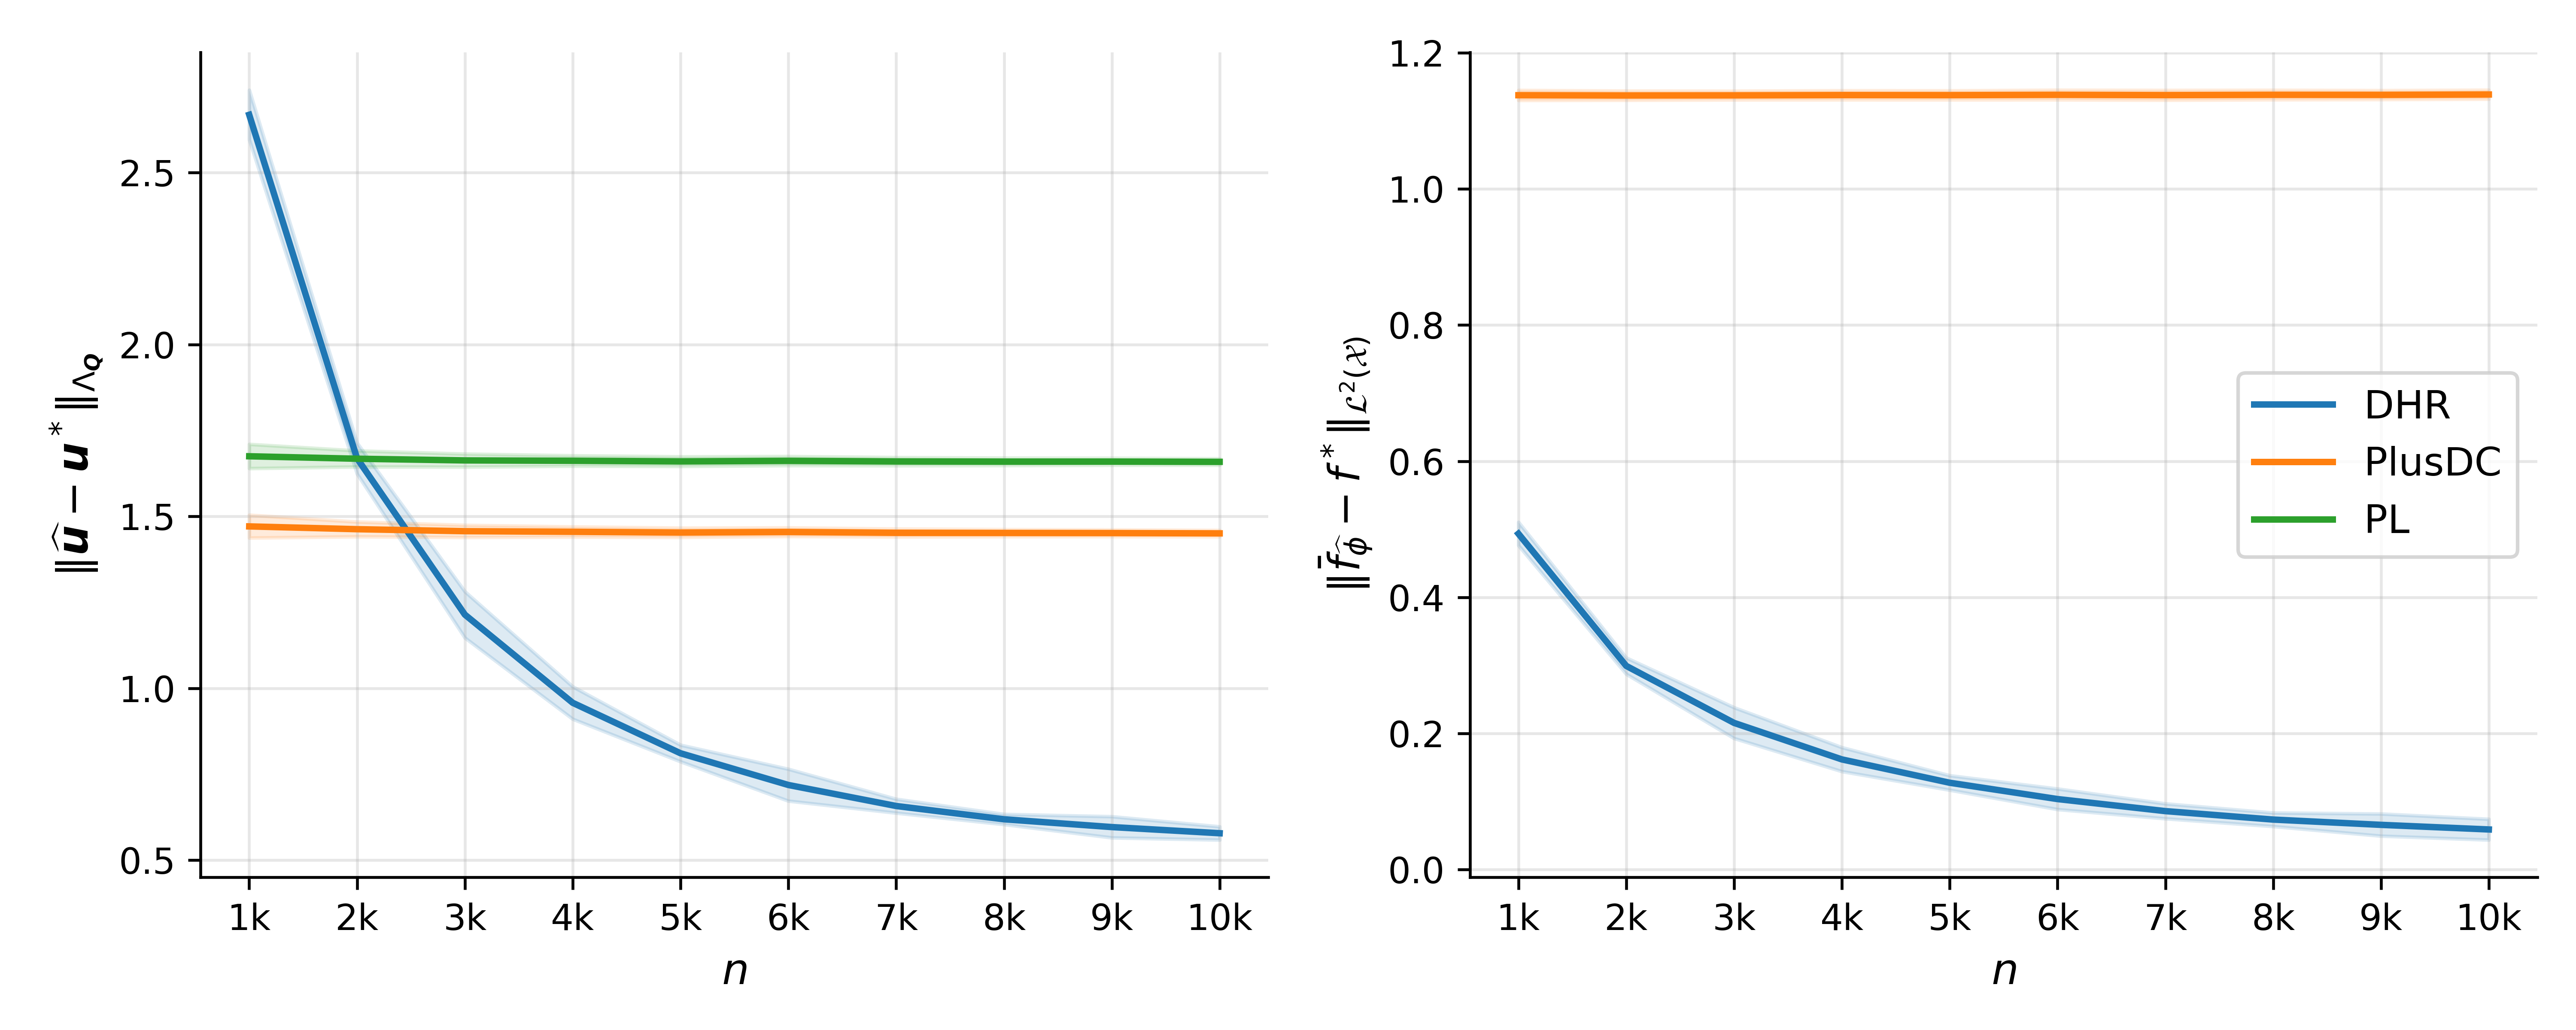
\includegraphics[width=\linewidth]{figure_benchmark.png}
    \caption{Trace plot of $\| \widehat{\boldsymbol{u}} -\boldsymbol{u}^{*} \|_{\Lambda_{\boldsymbol{Q}}}$ and 
    $\|\bar{f}_{\widehat{\phi}}-f^{*} \|_{\mathcal{L}^{2}(\mathcal{X})}$ under different methods. The shade represents one standard deviation over 300 replications. $\mathcal{L}^{2}(\mathcal{X})$ error for PL model is not available.}
    \label{fig:MDC}
\end{figure}

Figure \ref{fig:MDC} presents the results. The error curves for both PL and PlusDC plateau as $n$ grows, indicating a non-vanishing bias, while the latter achieves a lower utility estimation error by leveraging covariate information through linear approximation. However, the nonlinear component remains unrecoverable. In contrast, the DHR model exhibits steadily decreasing errors in both metrics, confirming that the semiparametric framework successfully captures complex covariate effects that linear specifications fail to capture.

\subsection{~Data processing and Feature Engineering}
We constructed the ATP match dataset from raw match-level records that contain match information, player profiles, and in-match statistics for both players. The data processing pipeline consisted of three main steps: variable transformation, missing-value imputation, and data filtering. Since some fields in the raw data were originally stored as strings, we first transformed them into numerical or categorical variables. To avoid data leakage, missing values for in-match statistics values were imputed in temporal order. Specifically, for each player, a missing value was replaced by that player’s historical median computed only from matches played before the current one. Finally, we removed matches that still lacked complete information after data imputation.

Based on the processed dataset, we then constructed features at three levels: match-level contextual variables, player-level profile attributes, and historical performance statistics. These features include match information such as ground type, ATP level, and match round; player profile variables such as handedness, height, age, and home advantage; and historical technical statistics aggregated over a rolling 3-month window before each match. Historical technical statistics summarize both a player's own recent performance and the aggregated performance statistics of all opponents that player faced within the same temporal window.

These features were subsequently encoded into fixed-dimensional covariate vectors suitable for model input. Categorical variables were transformed using one-hot encoding. Numerical variables were processed according to their type.
For historical technical statistics, proportion-type variables were transformed using a logit transformation and frequency-type variables were transformed using a logarithmic transformation. All remaining continuous numerical variables, including those in the player profile group, were retained in their original scale after appropriate rounding. A summary of all features and their corresponding transformations is provided in Table~\ref{tab:atp_features}. 

\begin{table}[t]
\centering
\scriptsize
\begin{tabular}{lllc}
\toprule
Variable & Group & Type & Transformation \\
\midrule
Ground type                       & MI               & categorical              & One-hot     \\
ATP level                         & MI               & categorical              & One-hot     \\
Match round                       & MI               & categorical              & One-hot     \\
Handedness                        & PP                  & categorical              & One-hot     \\
Height                            & PP                  & continuous   & --          \\
Age                               & PP                  & continuous   & --          \\
Seed rank                         & PP                  & discrete     & --          \\
Seed status                       & PP                  & categorical              & One-hot     \\
Home advantage                    & PP                  & categorical              & One-hot     \\
Recent number of matches                  & PP                  & discrete     & --          \\
Recent win rate                   & PP                  & continuous  & --          \\
Recent streak                     & TS & frequency    & $\log(x+1)$ \\
Recent tiebreaks                  & TS & frequency    & $\log(x+1)$ \\
Recent point streak               & TS & frequency    & $\log(x+1)$ \\
Recent receiver points            & TS & frequency    & $\log(x+1)$ \\
Recent service points             & TS & frequency    & $\log(x+1)$ \\
Recent break points converted     & TS & frequency    & $\log(x+1)$ \\
Recent first-serve return points  & TS & frequency    & $\log(x+1)$ \\
Recent return games played        & TS & frequency    & $\log(x+1)$ \\
Recent second-serve return points & TS & proportion   & Logit       \\
Recent aces                       & TS & frequency    & $\log(x+1)$ \\
Recent break points saved         & TS & proportion   & Logit       \\
Recent double faults              & TS & frequency    & $\log(x+1)$ \\
Recent first-serve rate           & TS & proportion   & Logit       \\
Recent first-serve points         & TS & proportion   & Logit       \\
Recent second-serve rate          & TS & proportion   & Logit       \\
Recent second-serve points        & TS & proportion   & Logit       \\
Recent service games played       & TS & frequency    & $\log(x+1)$ \\
\bottomrule
\end{tabular}
\caption{Summary of engineered features used in the ATP experiment.}
\label{tab:atp_features}
\end{table}




\subsection{~Implementation Details}
DHR and its Ablated model described in Section~\ref{sec:ATP} are implemented in Pytorch and trained on an Intel Xeon Gold 6330 CPU with 112 cores.  We repeat these models 30 times and the results are aggregated over 30 runs. The optimal hyperparameters are tuned through a grid search 
over the validation set. The search range is defined as follows: learning 
rate $\in \{0.001, 0.00075, 0.0005\}$, batch size $\in \{32, 64, 128, 256\}$, 
the number of hidden layers fixed at $3$, hidden dimension $\in \{16, 32\}$, 
and weight decay fixed at $0.0001$.

\subsection{~Additional Experimental Results}\label{appendix: anr}
We report additional numerical results in Figure~\ref{fig:additional results}. The deep model achieves the best Brier scores across all feature combinations and obtains the best or near-best test accuracy in most cases.

\begin{figure}[h]
  % Added [c] to align the image block vertically to the center
  \begin{subfigure}[b]{0.48\textwidth}
    \centering
    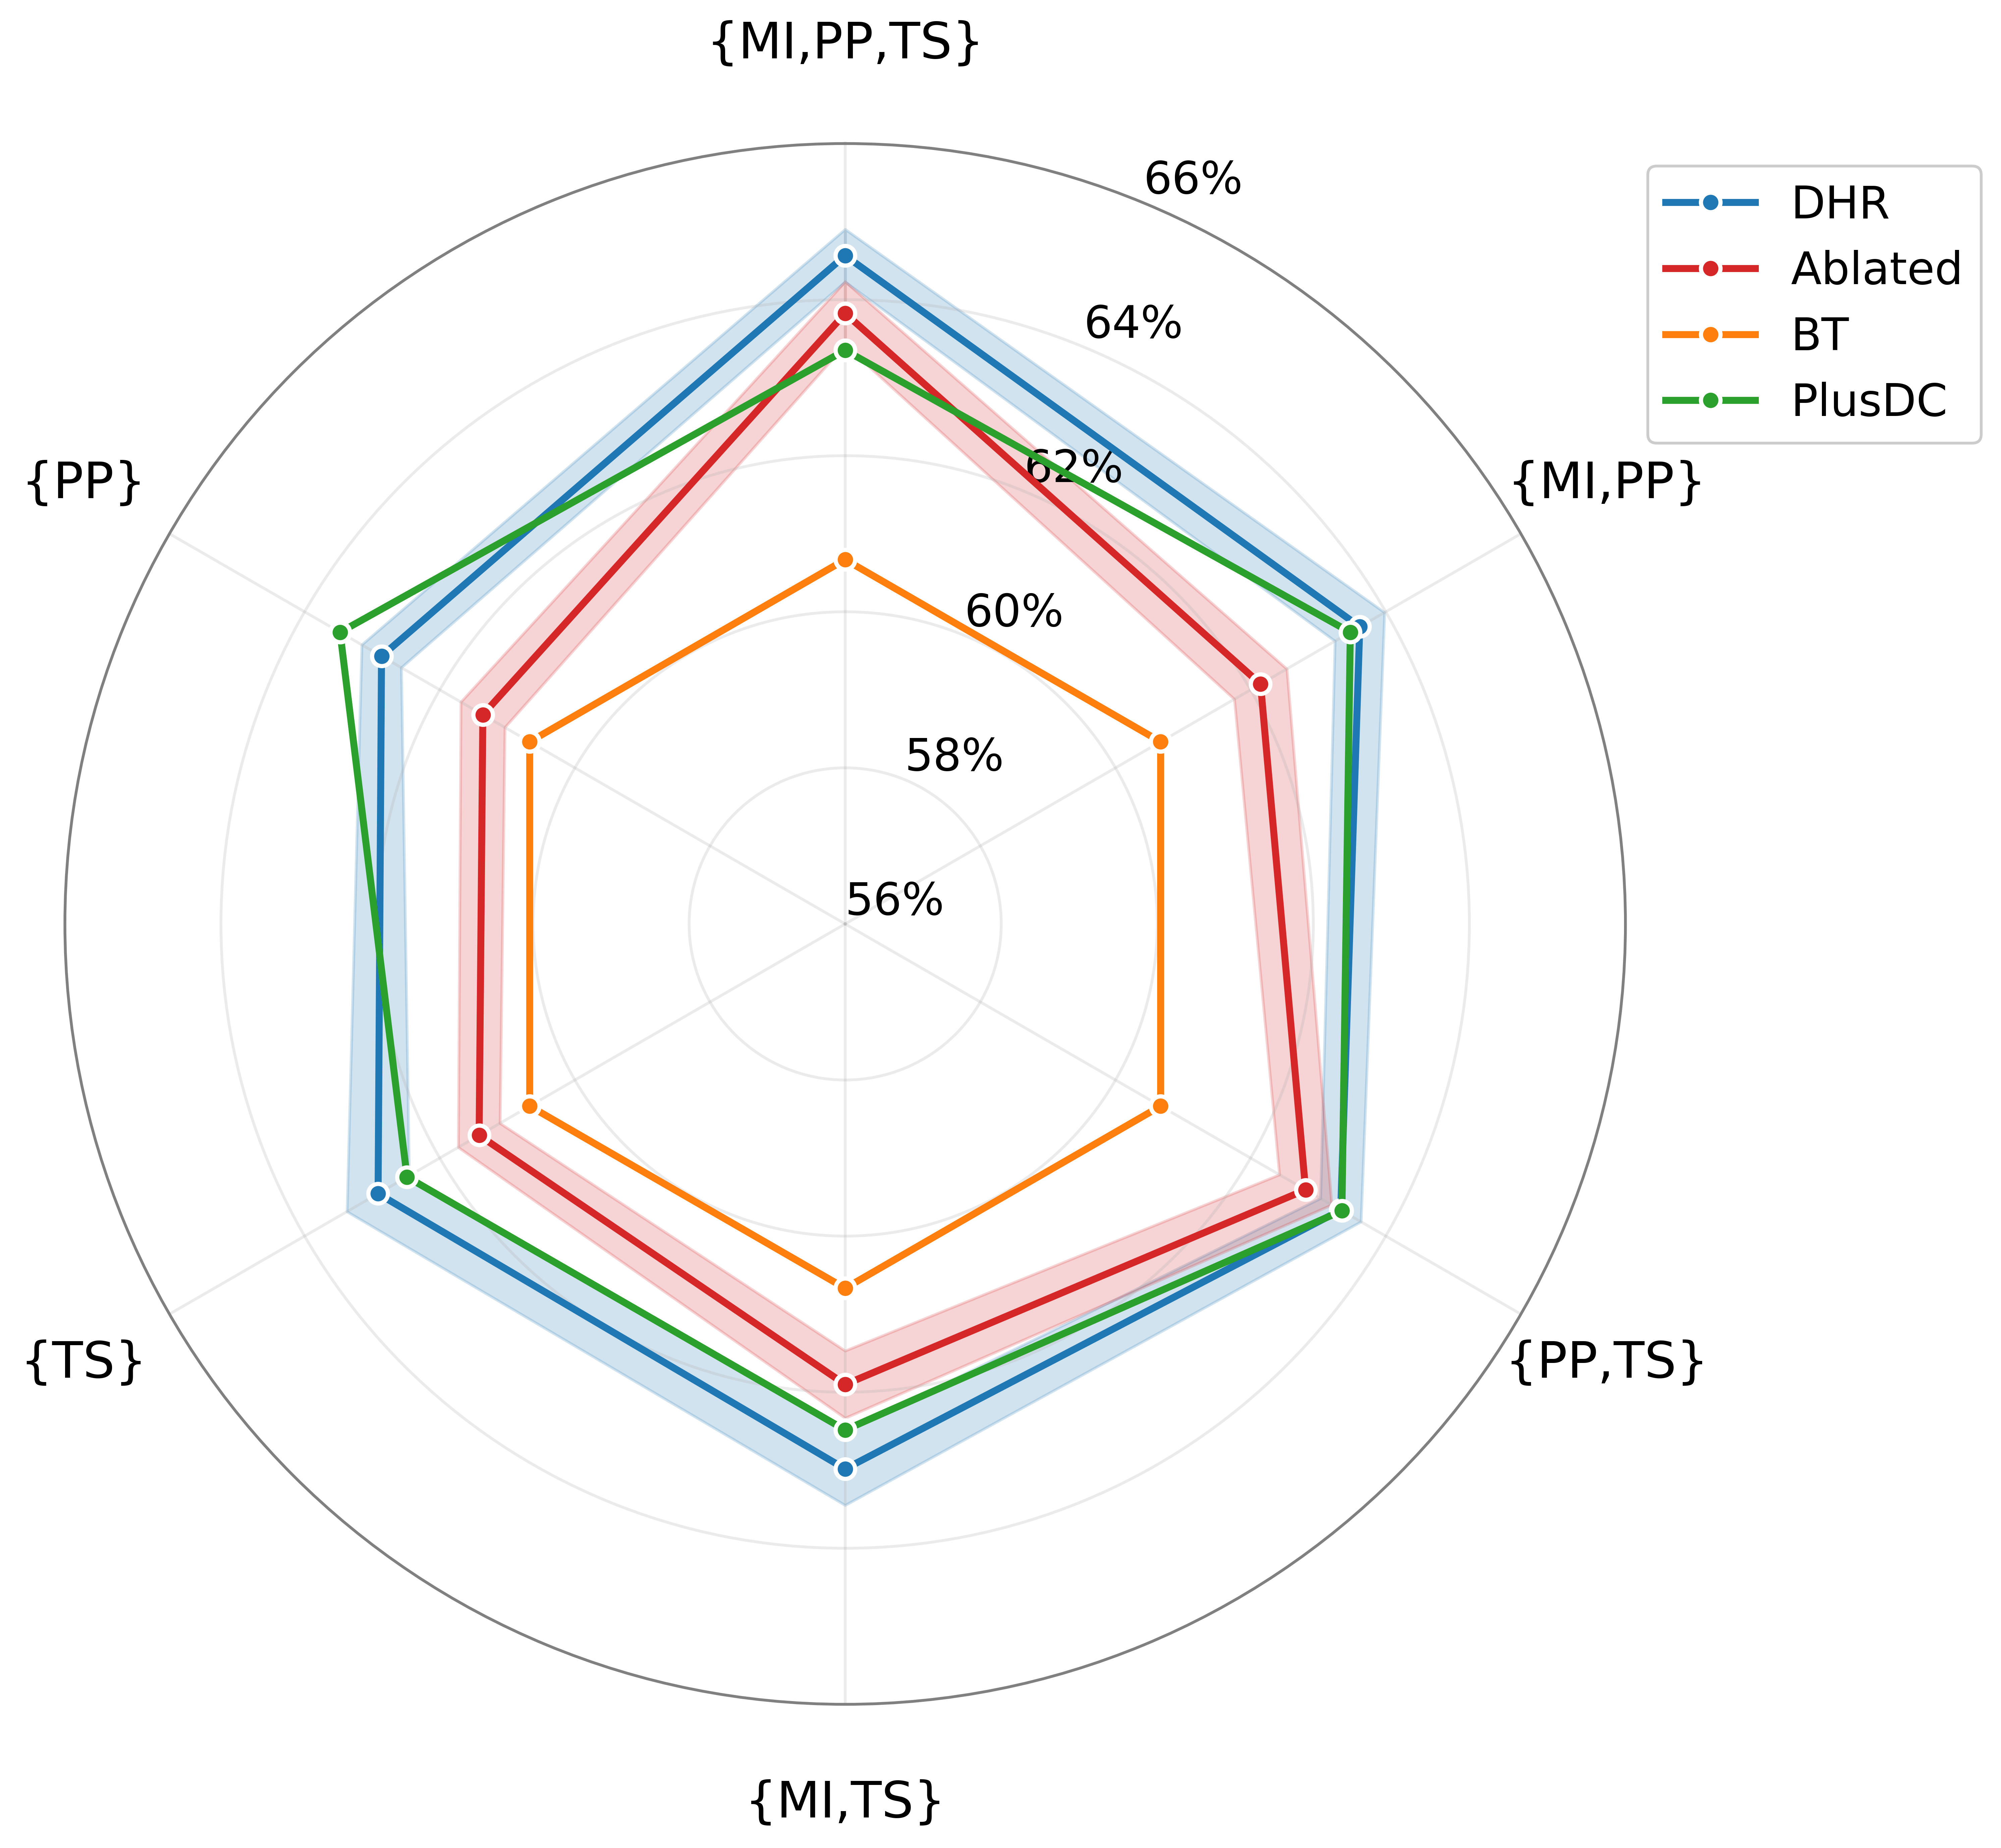
\includegraphics[width=\linewidth]{test_win_rate_radar_style2.png}
    \caption{}
    \label{fig:accurcy}
  \end{subfigure}
  \hfill 
    \begin{subfigure}[b]{0.48\textwidth}
        \centering
        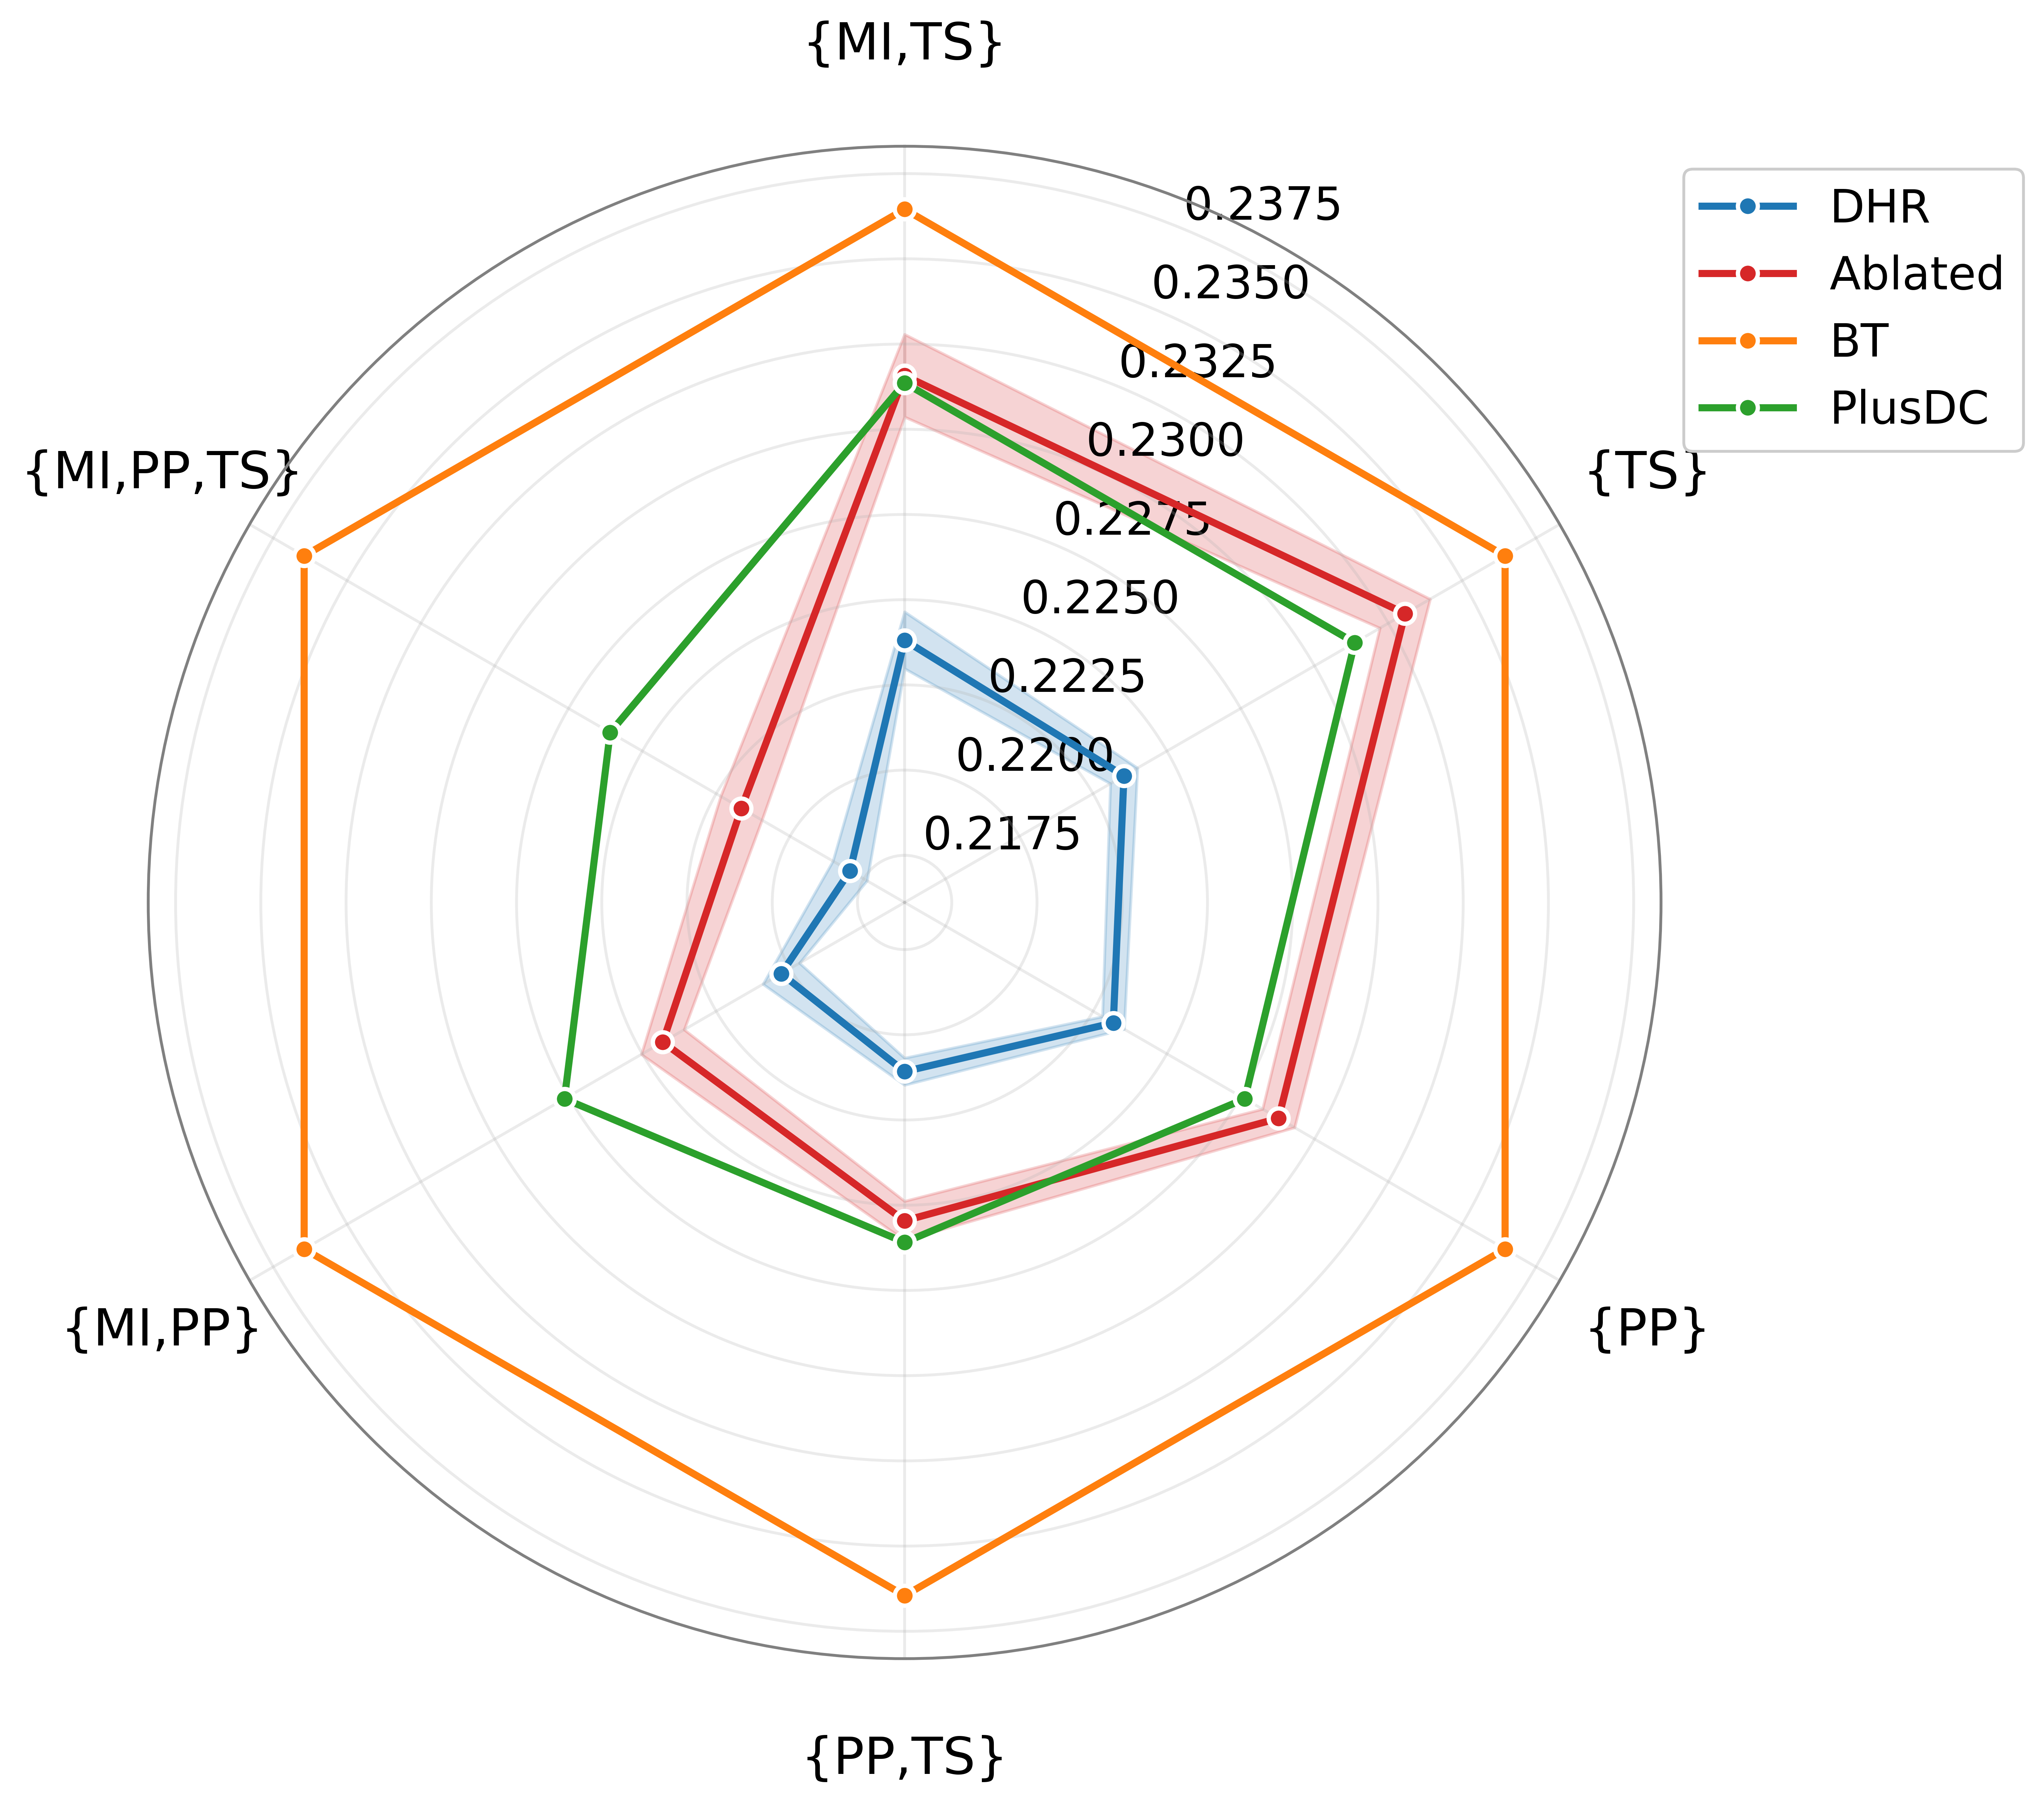
\includegraphics[width=\linewidth]{test_brier_score_radar_style2.png}
        \caption{}
        \label{fig:brier}
      \end{subfigure}
  \caption{Test performance of DHR versus baselines. (a) A radar chart depicting test accuracy across distinct feature combinations. (b) A radar chart depicting test Brier score across distinct feature combinations. The shades denote one standard deviation.}
  \label{fig:additional results}
\end{figure}


\bibliography{reference}

\end{document}
